% LaTeX source for book ``代数学方法'' in Chinese
% Copyright 2018  李文威 (Wen-Wei Li).
% Permission is granted to copy, distribute and/or modify this
% document under the terms of the Creative Commons
% Attribution 4.0 International (CC BY 4.0)
% http://creativecommons.org/licenses/by/4.0/

% To be included
\chapter{环论初步}\label{sec:ring}
环是具有加法和乘法两种二元运算的结构, 满足结合律, 分配律等习见的运算法则, 然而不要求乘法交换. 交换环的根本例子是整数环 $\Z$. 推而广之, 在数论中, 任意一个代数数域中的代数整数皆对加法和乘法构成交换环; 正是在这个脉络下, Hilbert 于 1897 年出版的《数论报告》中首次引进了环的术语, 其原文是德文 \textit{der Zahlring}, 即``数环''. 非交换环的根本例子是域上的 $n \times n$-矩阵环, 譬如 $n \times n$-实矩阵环 $M_n(\R)$. 综之, 环结构在数学中的份量一目了然.

交换环与非交换环无论在性质或研究视角上都有明显差异, 域和除环又各有其独特的方法论, 必须各辟专章讨论. 本章目的仅是铺陈共通的基本概念, 并间杂以具体的经典结果, 如: Wedderburn 小定理 \ref{prop:Wedderburn-little-thm}, 唯一分解性 \S\ref{sec:UFD} 以及对称多项式的初步理论 \S\ref{sec:symmetric-poly}; 这些结果还会在后续章节登场.

如不另作说明, 我们仅考虑含幺元的环, 而且一般假设环 $\neq \{0\}$. 为了避免悖论, 论及环范畴 $\cate{Ring}$ 时我们仍沿用约定 \ref{con:U-small}, 假定所论的环在集合论意义下都是``小''的.

\begin{wenxintishi}
	本章内容较偏于形式面向, 着眼于为后继章节搭建合适的框架, 前半部内容在一般的抽象代数课程多有涉及. 在 \S\ref{sec:Mobius} 介绍 Möbius 反演有双重目的, 一是顾及未熟悉经典 Möbius 反演公式的读者, 二是说明环论语言对计数组合学的应用; 习题中还会提供进一步的例子.

	对称多项式也是大学数学课程常涉及的内容, 我们在 \S\ref{sec:symmetric-poly} 引进的 Young 图处理手法既非最快也不是最简单的, 其用意是介绍一套应用范围更广的思考模式.
\end{wenxintishi}

\section{基本概念}\label{sec:ring-basics}
环是一种具备加, 减与乘法运算的代数结构, 亦可视为叠架在一个交换群(运算写作加法)上的乘法结构, 后一观点在理论上往往更为便利.

\begin{definition}\index{huan@环 (ring)}
	(含幺) \emph{环}是一组资料 $(R, +, \cdot)$, 其中
	\begin{enumerate}
		\item $(R, +)$ 是交换群, 二元运算用加法符号记作 $(a,b) \mapsto a+b$, 加法幺元记为 $0$, 称之为 $R$ 的加法群;
		\item 乘法运算 $\cdot: R \times R \to R$ 简记为 $a \cdot b = ab$, 满足下述性质: 对所有 $a, b, c \in R$,
		\begin{compactitem}
			\item $a(b+c) = ab+ac$, \; $(b+c)a = ba + ca$ \quad (分配律, 或曰双线性),
			\item $a(bc) = (ab)c$ \quad (乘法结合律);
		\end{compactitem}
		\item 存在元素 $1 \in R$ 使得对所有 $a \in R$ 皆有 $a \cdot 1 = a = 1 \cdot a$, 称作 $R$ 的(乘法)幺元.\index{yaoyuan}
	\end{enumerate}
	除去和幺元相关性质得到的 $(R, +, \cdot)$ 称作无幺环. 若子集 $S \subset R$ 对 $(+, \cdot)$ 也构成环, 并且和 $R$ 共用同样的乘法幺元 $1$, 则称 $S$ 为 $R$ 的子环, 或称 $R$ 是 $S$ 的环扩张或扩环.
\end{definition}

以上定义蕴涵了 $(R, \cdot)$ 构成幺半群, 故幺元 $1$ 是唯一的, 必要时标注为 $1_R$. 子环 $S \subset R$ 的定义相当于说 $(S, +)$ 为子群而 $(S, \cdot)$ 为子幺半群. 左乘映射 $b \mapsto ab$ 对每个 $a \in R$ 都是加法群 $(R, +)$ 的自同态, 故环论公理蕴涵 $a \cdot 0 = 0$; 同理 $0 \cdot a = 0$. 此外, $(-1)a + a = (-1 + 1) a = 0$ 蕴涵 $(-1)a = -a$; 同理 $a(-1) = -a$.

留意到满足 $1=0$ 的环只有一个元素 $0$, 称作\emph{零环}. 本章如不另作说明, 环皆指非零的含幺环, 并将 $(R, +, \cdot)$ 简记为 $R$, 其中对乘法可逆的元素全体记为 $R^\times$; 这和先前关于幺半群中可逆元的符号是一致的.\index[sym1]{$R^\times$}

\begin{definition}\index{xiangfanhuan@相反环 (opposite ring)}
	设 $R$ 为环, 定义其相反环 $R^\text{op} = (R, +, \odot)$, 其中仅乘法运算 $\odot$ 改为
	\[ a \odot b := ba, \quad a, b \in R. \]
	若 $R^\text{op}=R$ (即: $ab=ba$ 恒成立), 则 $R$ 称为\emph{交换环}. \index{jiaohuan}
\end{definition}

\begin{definition}\index{tongtai}
	设 $R, S$ 为环, 映射 $\varphi: R \to S$ 若满足下列条件则称为环同态: 对所有 $a, b \in R$
	\begin{itemize}
		\item $\varphi(a+b) = \varphi(a)+\varphi(b)$, 这相当于说 $\varphi$ 是加法群的同态;
		\item $\varphi(ab)=\varphi(a)\varphi(b)$;
		\item $\varphi(1_R) = 1_S$, 以上两条相当于说 $\varphi$ 是乘法幺半群的同态.
	\end{itemize}
	如去掉与 $1_R$, $1_S$ 相关的条件, 就得到无幺环之间的同态概念.
\end{definition}
由此可导出环的同构 (即可逆同态), 自同态, 自同构等概念, 与 \S\ref{sec:cat-and-morphism} 探讨范畴论时同一套路, 不再赘述.

一个同态 $\varphi$ 是同构当且仅当它是双射, $\varphi$ 的像 $\Image(\varphi)$ 是 $S$ 的子环. 对环同态依然有\emph{核} $\Ker(\varphi) := \varphi^{-1}(0)$ 的概念, 我们马上会看到同态的核无非是环的双边理想.\index{he}

\begin{example}\label{eg:matrix-ring}\index[sym1]{$M_n(R)$}
	非交换环的基本例子是矩阵环: 设 $n \in \Z_{\geq 1}$ 而 $R$ 为环, 定义矩阵环 $M_n(R)$ 使其元素为 $n \times n$ 阶矩阵
	\[ (a_{ij})_{1 \leq i,j \leq n} = \begin{pmatrix}
		a_{11} & \cdots & a_{1n} \\
		\vdots & & \vdots \\
		a_{n1} & \cdots & a_{nn}
	\end{pmatrix}, \quad \forall i,j,\; a_{ij} \in R \]
	加法, 乘法定义为习见的矩阵运算; 注意到这里不要求 $R$ 交换. 矩阵环的幺元是
	\[ 1 = \left( \begin{smallmatrix} 1_R & & \\ & \ddots & \\ & & 1_R \end{smallmatrix} \right). \]
\end{example}

\begin{example}\label{eg:End-ring}\index{zitongtaihuan@自同态环}
	设 $(A, +)$ 为交换群, 则 $A$ 的自同态集 $\End(A)$ 具有自然的环结构: 自同态的合成给出乘法 $\phi \psi = \phi \circ \psi$, 其中 $\phi, \psi \in \End(A)$, 而加法可以``逐点地''定义成
	\[ \phi + \psi: a \longmapsto \phi(a) + \psi(a). \]
	容易验证这使 $(\End(A), +, \cdot)$ 成环, 幺元是 $\identity_A$.
\end{example}

接着考虑环的商. 设 $R$ 为环, 这里的思路和 \S\ref{sec:homomorphism} 类似: 给定集合 $R$ 上的等价关系 $\sim$, 试问在什么条件下能赋予 $R/\sim$ 典范的环结构, 使得商映射 $R \to R/\sim$, $r \mapsto [r]$ 为环同态? 环同态首先必是加法群的同态, 因而等价关系由一个加法子群 $I \subset R$ 确定, 使得对所有 $r, r' \in R$ 有
\[ (r \sim r') \iff (r-r' \sim 0) \iff (r-r' \in I). \]

现在计入乘法, $\sim$ 须满足条件
\[ (r \sim r') \wedge (s \sim s') \implies (rs \sim r's'). \]
由环的公理易知 $rs - r's' = r(s-s') + (r-r')s'$. 因此我们的条件化归为: $\forall r \in R$, 有 $rI \subset I$, $Ir \subset I$; 这里
\begin{align*}
	rI & := \{ra : a \in I\} \subset R, \\
	Ir & := \{ar : a \in I\} \subset R,
\end{align*}
两者皆为 $R$ 的加法子群. 事实上由 $R$ 含幺元可知以上条件等价于 $IR = I = RI$. 于是我们提炼出以下定义.

\begin{definition}\label{def:ideals}\index{lixiang@理想 (ideal)}
	设 $R$ 为环, $I \subset R$ 为加法子群.
	\begin{compactenum}[(i)]
		\item 若对每个 $r \in R$ 皆有 $rI \subset I$, 则称 $I$ 为 $R$ 的\emph{左理想};
		\item 若对每个 $r \in R$ 皆有 $Ir \subset I$, 则称 $I$ 为 $R$ 的\emph{右理想};
		\item 若 $I$ 兼为左, 右理想, 则称作\emph{双边理想}.
	\end{compactenum}
	满足 $I \neq R$ 的左, 右或双边理想称为真理想. 交换环的左, 右理想不分, 简称为理想.
\end{definition}
关于加法子群的前提可以放宽为 $I$ 对加法封闭且非空, 因为 $(-1)r = -r$. 理想具有以下几种最简单的运算.
\begin{itemize}
	\item 设 $I_1$, $I_2$ 为 $R$ 的左理想 (或右理想, 双边理想), 则 $I_1 + I_2$ 与 $I_1 \cap I_2$ 亦然. 推而广之, 对于任意一族 $R$ 的左理想 (或右理想, 双边理想) $\{ I_t: t \in T \}$, 定义其和
		\[ \sum_{t \in T} I_t := \left\{ r_{t_1} + \cdots + r_{t_n} :
		\begin{array}{l}
			n \in \Z_{\geq 1}, \; t_1, \ldots, t_n \in T, \\
			\forall 1 \leq j \leq n, \; r_{t_j} \in I_{t_j}
		\end{array} \right\}, \]
		对 $T = \emptyset$ 约定空和为 $\{0\}$, 则 $\sum_{t \in T} I_t$ 也是左理想 (或右理想, 双边理想). 同理, 当 $T \neq \emptyset$ 时, 类似断言对交 $\bigcap_{t \in T} I_t$ 也成立.
	\item 对 $R$ 的任意子集 $S$, 定义由 $S$ 生成的左理想 (或右理想, 双边理想) 为包含 $S$ 的最小的左理想 (或右理想, 双边理想), 即 $\bigcap_{I \supset S} I$, 其中 $I$ 取遍左理想 (或右理想, 双边理想).
	\item 设 $I$ 为双边理想, $S$ 为子环, 则 $S+I$ 亦为子环.
	\item 设 $S$ 为子环, $I$ 在 $R$ 中为左理想 (或右理想, 双边理想, 子环), 则 $S \cap I$ 在 $S$ 中亦然.
	\item 定义双边理想 $I$, $J$ 的积 $IJ$ 为由子集 $\{xy : x \in I,\; y \in J\}$ 生成的理想, 注意到 $IJ$ 的元素能表为这些 $xy$ 的和. 积运算具有以下简单性质,
		\begin{gather*}
			IJ \subset I \cap J \subset I+J, \\
			(\sum_{t \in T} I_t) J = \sum_{t \in T} (I_t J), \quad J(\sum_{t \in T} I_t) = \sum_{t \in T} J I_t, \\
			I(JK) = (IJ)K.
		\end{gather*}
		利用最后一条结合律, 可定义有限多个理想的积 $I_1 \cdots I_n$; 理想 $I$ 的幂次可递归地按 $I^0 = R$ 和 $I^k = I \cdot I^{k-1}$ 来定义, 此处 $k \in \Z_{\geq 1}$. 
\end{itemize}
一般将有限个元素 $r_1, \ldots, r_n \in R$ 生成的双边理想记为 $\lrangle{r_1, \ldots, r_n}$. 在交换环的情形也习惯写作 $(r_1, \ldots, r_n)$.

\begin{definition}\index{shang}
	设 $I$ 为 $R$ 的双边理想, 赋予加法群 $R/I$ 乘法运算如下
	\[ (r+I) \cdot (s+I) := (rs + I), \quad r, s \in R. \]
	则 $R/I$ 构成一个环, 称为 $R$ 模 $I$ 的\emph{商环}. 商映射 $R \twoheadrightarrow R/I$ 称为\emph{商同态}.
\end{definition}
我们在定义 \ref{def:ideals} 前的讨论中业已说明了 $R/I$ 确实成环, 其幺元是 $1_{R/I} = 1_R + I$; 而且从定义立得 $R \twoheadrightarrow R/I$ 确实为同态. 须注意到 $R/I$ 是零环当且仅当 $I=R$, 我们通常仅考虑 $I$ 是真理想的情形. 取商 $R/I$ 的操作有时也叫作 $\bmod \;I$.

\begin{example}\label{eg:Z-pid}
	设 $n \in \Z$, 则 $n\Z$ 是 $\Z$ 的理想. 当 $n \neq 0$ 时商环 $\Z/n\Z$ 中的运算无非就是数论中的同余类操作. 反过来看, 任意理想 $I \subset \Z$ 必为 $I=n\Z$ 的形式: $I=\{0\}$ 时自不待言, 如非零则取 $I \cap \Z_{> 0}$ 中的极小元 $n$, 由带余除法知 $I$ 中元素必被 $n$ 整除; 如要求 $n \geq 0$, 则 $n$ 是唯一确定的. 这表明 $\Z$ 是稍后将介绍的主理想环 (定义 \ref{def:PID})的初等例子.
\end{example}

商环满足一些与商群共通的性质如下, 证明和群的情形如出一辙, 留作练习.
\begin{proposition}\label{prop:quotient-ring-univ-prop}
	设 $I \subset R$ 为双边理想, 则对任意环同态 $\varphi: R \to R'$ 满足 $\varphi(I)=0$ 者, 存在唯一的同态 $\bar{\varphi}: R/I \to R'$ 使得下图交换.
	\[ \begin{tikzcd}[row sep=small]
		R \arrow[r, "\varphi"] \arrow[d] & R' \\
		R/I \arrow[ur, "{\exists! \,\bar{\varphi}}"'] &
	\end{tikzcd} \]
\end{proposition}

\begin{proposition}\label{prop:1st-homomorphism-ring}
	设 $\varphi: R \to R'$ 为环同态, 则 $\Ker(\varphi) := \varphi^{-1}(0)$ 是 $R$ 的双边理想, 且诱导同态 $\bar{\varphi}: (R/I) \to \Image(\varphi)$ 是环同构.
\end{proposition}

接着观察到对任意环同态 $\varphi: R_1 \to R_2$, 理想间有相应的原像映射:
\begin{equation}\label{eqn:ideal-preimage}\begin{aligned}
	\left\{ R_2 \text{的双边理想} \right\} & \longrightarrow \left\{ R_1 \text{的双边理想} \right\} \\
	I_2 & \longmapsto \varphi^{-1}(I_2).
\end{aligned}\end{equation}
此映射满足
\[ I_2 \subset I'_2 \implies \varphi^{-1}(I_2) \subset \varphi^{-1}(I'_2). \]
如取 $\varphi$ 为子环的包含映射 $R_1 \hookrightarrow R_2$, 便得到 $I_2 \mapsto I_2 \cap R_1$. 下面考虑另一个极端, 即商同态或满同态(回忆命题 \ref{prop:1st-homomorphism-ring})的情形.

\begin{proposition}\label{prop:2nd-homomorphism-ring}
	设 $\varphi: R_1 \to R_2$ 是满的环同态. 则 \eqref{eqn:ideal-preimage} 诱导出双射
	\[ \begin{tikzcd}[row sep=tiny]
		\left\{ \text{双边理想}\;  I_2 \subset R_2  \right\} \arrow[leftrightarrow, r, "1:1"] & \left\{ \text{双边理想}\; I_1 \subset R_1 : I_1 \supset \Ker(\varphi)  \right\} \\
		I_2 \arrow[mapsto, r] & \varphi^{-1}(I_2) \\
		\varphi(I_1) & I_1 \arrow[mapsto, l].
	\end{tikzcd} \]
	而且合成同态 $R_1 \xrightarrow{\varphi} R_2 \twoheadrightarrow R_2/I_2$ 诱导出环同构 $R_1/\varphi^{-1}(I_2) \rightiso R_2/I_2$.
\end{proposition}

接着考虑子环 $S \subset R$ 及双边理想 $I \subset R$. 合成同态 $S \hookrightarrow R \twoheadrightarrow R/I$ 的像为 $R/I$ 的子环 $(S+I)/I$, 它的核显然是 $I \cap S$. 以下证明与群的情形同一套路, 是故略去.
\begin{proposition}\label{prop:3rd-homomorphism-ring}
	设 $S$ 是 $R$ 的子环而 $I$ 是 $R$ 的双边理想, 则合成同态 $S \twoheadrightarrow (S+I)/I$ 诱导的环同态
	\[ \theta: S/I \cap S \to (S+I)/I \]
	乃是同构.
\end{proposition}

和左理想或右理想相关的构造将在模论部分统一处理.

\section{几类特殊的环}
设 $R$ 为环, 以下皆假设 $R$ 非零. 对任意 $x \in R$, 定义其\emph{中心化子}
\[ Z_R(x) := \left\{ r \in R : rx=xr \right\}; \]
环 $R$ 的\emph{中心} 定为\index{zhongxin}\index[sym1]{$Z_R$}
\[ Z_R := \left\{r \in R : \forall s \in R, rs=sr \right\} = \bigcap_{x \in R} Z_R(x). \]
这些都是 $R$ 的子环, 而且 $Z_R$ 是交换环.

既然 $R$ 对乘法构成幺半群, 故可定义其中元素的左逆与右逆. 设 $r \in R$ 非零, 若 $r$ 可逆, 其逆记为 $r^{-1}$; 全体可逆元构成的乘法群记为 $R^\times$. 若存在 $r' \neq 0$ 使得 $rr'=0$ 则称 $r$ 为\emph{左零因子}; 条件改作 $r'r=0$ 则称\emph{右零因子}. 为 $R$ 中左或右零因子的元素统称为\emph{零因子}. 元素 $r \in R \smallsetminus \{0\}$ 非左零因子当且仅当 $r$ 的左乘满足消去律, 这是由于 $ra=rb \iff r(a-b)=0$; 右零因子的情形类似.\index{lingyinzi@零因子 (zero divisor)}

由于环对加法成群, 对其中元素可取任意整数倍: 如 $(-1)r = -r$, $nr = \underbracket{r + \cdots + r}_{n\; \text{项}}$, $(-n)r = nr$ 等等 (设 $n \geq 0$). 不难验证映射
\begin{equation}\label{eqn:ring-struct-morphism}\begin{aligned}
	\Z & \longrightarrow R \\
	a & \longmapsto a \cdot 1_R
\end{aligned}\end{equation}
为环同态; 这也是从 $\Z$ 到 $R$ 的唯一同态, 像包含于 $Z_R$. 由命题 \ref{prop:1st-homomorphism-ring} 和例 \ref{eg:Z-pid} 知其像必同构于某个 $\Z/p\Z$, 其中 $p \in \Z_{\geq 0}$ 是唯一的. 此时必有 $p \neq 1$, 否则在 $R$ 中 $1=0$ 将导致 $R$ 是零环. 记此数 $p$ 为 $\text{char}(R)$.

\begin{definition}\label{def:ring-characteristic}\index{tezheng@特征 (characteristic)}\index[sym1]{char@$\text{char}(R)$}
	设 $R$ 非零环, 定义其\emph{特征}为上述的 $\text{char}(R)$. 
\end{definition}
如果 $R$ 中没有非零的零因子, 则 $\Z/p\Z$ 亦然, 后者成立当且仅当 $p=0$ 或素数. 以下的公式在域论中格外有用: 设交换环 $R$ 的特征为素数 $p$, 则
\begin{equation}\label{eqn:freshmen-dream}
	(u+v)^{p^m} = u^{p^m} + v^{p^m}, \quad u, v \in R, \; m \geq 0;
\end{equation}
这是 $R$ 上二项式定理和引理 \ref{prop:Wielandt-lemma} 的直接应用.

\begin{definition}\index{zhenghuan@整环 (integral domain)}
	无非零的零因子的交换环称为\emph{整环}.
\end{definition}

\begin{definition}\label{def:field}\index{chuhuan@除环 (division ring)}\index{yu@域 (field)}
	若环 $R$ 中的每个非零元皆可逆, 则称 $R$ 为\emph{除环}. 交换除环称为\emph{域}.
\end{definition}
按本节的约定, 除环不能是零环; 某些文献将除环称作体.

\begin{example} \index[sym1]{F_q@$\F_q$}
	设 $p$ 为素数, 则商环 $\Z/p\Z$ 是域, 一般记为 $\F_p$. 诚然, 若 $x \in \Z$ 和 $p$ 互素, 则辗转相除法表明 $xy + pz = 1$ 有整数解 $y,z$, 因而 $y+p\Z$ 给出 $x+p\Z$ 的乘法逆元.
\end{example}
除环 $D$ 中可作除法, 故存在包含 $1$ 的最小子域, 称为 $D$ 的\emph{素子域}; 当 $\text{char}(D)=0$ 时, $\Z \hookrightarrow D$, 故其素子域同构于有理数域 $\Q$; 若 $\text{char}(D)=p > 0$, 其素子域是上述之 $\F_p$. \index{suziyu@素子域 (prime subfield)}

环上的拓扑, 几何结构或有限性等条件往往与其代数性质有着微妙的关系. 下述两个结果是绝佳范例. 定理 \ref{prop:Wedderburn-little-thm} 的证明略需一些多项式和初等数论的知识.

\begin{proposition}
	有限环 $D$ 若无非零的零因子, 则 $D$ 必为除环. 
\end{proposition}
\begin{proof}
	设 $x \in D$, $x \neq 0$. 由条件可知从 $D$ 到自身的左乘映射 $L_x: r \mapsto xr$ 为单射. 因为 $D$ 有限, $L_x$ 自动是双射, 故存在 $x' \in R$ 使得 $xx'=1$, 即 $x$ 右可逆. 同理, 考虑右乘映射可知 $x$ 左可逆. 因而 $x \in D^\times$.
\end{proof}

\begin{theorem}[Wedderburn 小定理]\label{prop:Wedderburn-little-thm}\index{Wedderburn 小定理}
	有限除环必为域.
\end{theorem}
\begin{proof}[E.\ Witt]
	设 $D$ 为有限除环. 对任意 $r \in D^\times$, 应用 $r^{\pm 1}$ 在 $D$ 上的共轭作用可知对任意 $x \in D$,
	\[ xr = rx \iff r^{-1}x = xr^{-1}. \]
	由之得到两条推论: 第一, $Z_D(x) \smallsetminus \{0\}$ 对取逆封闭, 因而 $Z_D(x)$ 是子除环; 第二, $Z_D \smallsetminus \{0\}$ 也对取逆封闭, 从而 $Z_D$ 是域. 以下置 $F := Z_D$, 记其基数为 $q \in \Z_{\geq 2}$.

	注意到 $D$ 在 $F$ 的乘法作用下构成 $F$-向量空间, 由假设知 $n := \dim_F D$ 有限. 下面证明 $n = 1$, 由此立见 $D = F$ 交换.

	对乘法群 $D^\times = D \smallsetminus \{0\}$ 的共轭作用应用引理 \ref{prop:orbit-decomp}, 可得
	\begin{equation}\label{eqn:Wedderburn-little}
		q^n - 1 = \underbracket{q-1}_{= |F^\times|} + \sum_x (D^\times : Z_D(x)^\times)
	\end{equation}
	其中 $x$ 取遍 $D^\times \smallsetminus F^\times$ 在共轭作用下的一组代表元. 注意到 $Z_D(x)$ 也是 $F$-向量空间, 维数记为 $n(x) \in \Z_{\geq 1}$, 故 $n(x) < n$ 而
	\[ (D^\times : Z_D(x)^\times) = \dfrac{q^n - 1}{q^{n(x)} - 1}. \]
	兹断言 $n(x) \mid n$. 根据初等数论的结果或稍后的例 \ref{eg:gcd-cyclotomic}, 可知 $q^n - 1$ 和 $q^{n(x)} - 1$ 的最大公因子是 $q^{(n, n(x))} - 1$, 因此 $\frac{q^n - 1}{q^{n(x)} - 1} = (D^\times : Z_D(x)^\times) \in \Z$ 导致所求之 $n(x) \mid n$. 另一条途径则是将 $D$ 视为除环 $Z_D(x)$ 上的左向量空间, 那么 $n/n(x) = \dim_{Z_D(x)} D$; 这需要 \S\ref{sec:vector-space} 的理论, 留给读者探究.
	
	下面将应用分圆多项式的理论: 这是一族最高次项系数为 $1$ (简称首一) 的整系数多项式 $\Phi_r(X)$, $r \in \Z_{\geq 1}$, 使得\index{fenyuanduoxiangshi@分圆多项式 (cyclotomic polynomial)}
	\begin{gather*}
		X^m - 1 = \prod_{r \mid m} \Phi_r(X), \quad m \in \Z_{\geq 1}, \\
		\deg \Phi_r = \varphi(r) := |(\Z/r\Z)^\times| \qquad \text{(Euler 函数)}
	\end{gather*}
	恒成立. 直接的定义是
	\begin{align*}
		\Phi_m(X) & = (X^m - 1) \cdot \prod_{\substack{p: \text{素数} \\ p \mid m}} (X^{m/p} - 1)^{-1} \cdot \prod_{\substack{p \neq q: \text{素数} \\ pq \mid m}} (X^{m/pq} - 1) \cdots \\
		& = \prod_{d \mid m} (X^d - 1)^{\mu(m/d)}, \\
		\deg \Phi_m & = \sum_{d \mid m} d \mu\left( \frac{m}{d} \right) = \sum_{h \mid m} \frac{m}{h} \cdot \mu(h) \\
		& = \varphi(m) \qquad \because \text{初等数论, 或 \eqref{eqn:Euler-phi-sum}};
	\end{align*}
	其中 $\mu$ 表 Möbius 函数
	\[ \mu(d) = \begin{cases}
		(-1)^{(d \;\text{的素因子个数})}, & d \;\text{无 $1$ 之外的平方因子} \\
		0, & d \; \text{有平方因子} \neq 1.
	\end{cases}\]
	由于在整系数多项式环中 $X^{(a,b)}-1$ 是 $X^a - 1$ 和 $X^b - 1$ 的最大公因子 (例 \ref{eg:gcd-cyclotomic}), 这般定义的 $\Phi_m(X)$ 确实是首一整系数多项式, 它实际是运用容斥原理从 $X^m - 1$ 移除所有来自 $X^d - 1$ ($d \mid m, d \neq m$) 的首一因子后的硬核; 我们将在 \S\ref{sec:Mobius} 讨论 Möbius 反演的一般框架, 并在例 \ref{eg:Mobius-classical} 回顾这里用上的经典版本 (精确地说是其``乘性''情形). 分圆多项式的系统性研究是 \S\ref{sec:cyclotomic-ext} 的任务.

	在复数域 $\CC$ 上 $\Phi_m(X)$ 可分解为 $\prod_\zeta (X-\zeta)$, 其中 $\zeta$ 取遍 $\CC^\times$ 中的 $m$ 次单位原根. 因为 $n(x) \mid n$ 而 $n(x) < n$, 我们有整系数首一多项式之间的整除关系
	\[ \Phi_n(X) \mid X^n - 1, \quad \Phi_n(X) \mid \prod_{\substack{d \mid n \\ d \nmid n(x)}} \Phi_d(X) = \frac{X^n - 1}{X^{n(x)} - 1}; \]
	上式也可以透过在 $\CC$ 上作分解来证明. 代值 $X \leadsto q \in \Z$ 以后可见 \eqref{eqn:Wedderburn-little} 中的 $q^n-1$ 及每一项 $\frac{q^n - 1}{q^{n(x)} - 1}$ 都被 $\Phi_n(q)$ 整除, 因而 $\Phi_n(q)  \mid  q-1$. 另一方面, 假若 $n>1$, 则对每个 $\CC^\times$ 中的 $n$ 次单位原根 $\zeta$ 皆有
	\[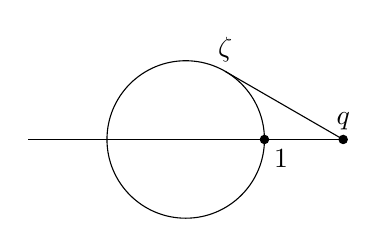
\begin{tikzpicture}[baseline=(O)]
		\draw (0,0) circle [radius=1cm];
		\draw (-2,0) -- (2,0);
		\coordinate (O) at (0:1cm); \coordinate (Q) at (2,0);  \coordinate (Z) at (60:1cm);
		\node[below right] at (O) {$1$}; \draw[fill=black] (O) circle [radius=1.5pt]; 
		\node[above] at (Q) {$q$}; \draw[fill=black] (Q) circle [radius=1.5pt];
		\node[above] at (Z) {$\zeta$};
		\draw (Q) -- (Z);
	\end{tikzpicture} \qquad
	\implies \quad |q-\zeta| > q-1 \geq 1.
	\]
	于是 $|\Phi_n(q)| = \prod_\zeta |q-\zeta| > q-1$, 导出矛盾.
\end{proof}

非交换除环的发现甚晚, 可稽的最早例子是 W.\ Hamilton 于 1843 年发现的\emph{四元数代数}. 以后探讨有限维代数时将给出构造这类除环的一些系统性的方法.
\begin{example}[四元数]\label{eg:Hamilton-quaternion}\index{siyuanshu@四元数 (quaternion)}\index[sym1]{H@$\mathbb{H}$}
	考虑以 $1, i, j, k$ 为基的实向量空间 $\mathbb{H} := \R 1 \oplus \R i \oplus \R j \oplus \R k$. 其上具有良定的乘法使得 $\mathbb{H}$ 成环并满足:
	\begin{itemize}
		\item 乘法 $(x,y) \mapsto xy$ 是 $\mathbb{H}$ 上的双线性映射;
		\item $1$ 是乘法单位元, 故我们可将 $\R$ 等同于 $\R \cdot 1$ 嵌入 $Z_{\mathbb{H}}$;
		\item $i^2 = j^2 = -1$;
		\item $ij=k=-ji$.
	\end{itemize}
	由此可以推导出 $k^2 = -1$, $jk=i=-kj$, $ki=j=-ik$. 细节留给读者. 由向量空间结构和前两条性质, 我们也说 $\mathbb{H}$ 是一个 ``$\R$-代数'', 定义 \ref{def:algebra-naive} 将有详细解释. 此外亦可将复数域 $\CC = \R \oplus \R i$ 嵌入 $\mathbb{H}$. 下面验证 $\mathbb{H}$ 是除环: 如定义共轭运算
	\[ z = a + bi + cj + dk \longmapsto \bar{z} = a - bi -cj -dk \]
	则有性质 $\overline{z w} = \bar{w}\bar{z}$, $z\bar{z} = \bar{z}z = a^2 + b^2 + c^2 + d^2 \in \R$, 由此可得
	\[ z^{-1} = (z\bar{z})^{-1} \bar{z} = (\underbracket{a^2 + b^2 + c^2 + d^2}_{\neq 0})^{-1} \bar{z}, \quad z \in \mathbb{H} \smallsetminus \{0\}. \]
	这里用到的关键性质可归结为 $a^2 + b^2 + c^2 = -1$ 在实数域 $\R$ 中无解, 更强的陈述是 $-1$ 在 $\R$ 中非平方和; 具后一条件的域称作形实域, 它们在域论, 二次型和模型论等研究中是饶富兴味的对象, 见 \cite[\S 9.1]{Feng17}. \index{moxinglun}
\end{example}

\section{交换环初探}\label{sec:comm-ring-intro}
交换环的理论与一般的非交换情形面貌迥异, 一方面体现于交换环所独有的一些概念与技术, 另一方面则归因于交换环在代数几何, 代数数论及代数组合学等领域中的关键地位. 本节目的仅在铺陈基本概念, 包括交换环的局部化, 较深入的研究将另辟专章讨论.

本节只论含幺交换环, 故理想不分左右.

\begin{definition}\label{def:ring-ideal}\index{lixiang!素理想 (prime ideal)}\index{lixiang!极大理想 (maximal ideal)}
	环 $R$ 的真理想 $I$ 称为
	\begin{compactitem}
		\item \emph{素理想}, 如果 $xy \in I$ 蕴涵 $x \in I$ 或 $y \in I$;
		\item \emph{极大理想}, 如果 $I \neq R$ 且不存在严格包含 $I$ 的理想.
	\end{compactitem}
	分别记 $R$ 中素理想和极大理想所成的集合为 $\Spec R$ 与 $\MaxSpec R$, 称为 $R$ 的素谱和极大理想谱. \index[sym1]{Spec@$\Spec$}\index[sym1]{MaxSpec@$\MaxSpec$}
\end{definition}
对任意环都能对左, 右和双边理想定义极大性的概念, 但用途不如交换情形来得广泛.

\begin{lemma}\label{prop:Spec-pullback}
	对任意环同态 $\varphi: R_1 \to R_2$, 式 \eqref{eqn:ideal-preimage} 映素理想为素理想; 换言之, 由 $\varphi$ 导出映射
	\begin{align*}
		\varphi^\sharp: \Spec R_2 & \longrightarrow \Spec R_1 \\
		I_2 & \longmapsto \varphi^{-1}(I_2).
	\end{align*}
	以范畴语言诠释, 映射
	\begin{align*}
		R & \longmapsto \Spec R, \\
		[\varphi: R_1 \to R_2] & \longmapsto [\varphi^\sharp: \Spec R_2 \to \Spec R_1]
	\end{align*}
	定义出函子 $\Spec: \cate{CRing}^\text{op} \to \cate{Set}$, 其中 $\cate{CRing}$ 表示交换环所成的范畴.
\end{lemma}
\begin{proof}
	设 $I_2$ 为 $R_2$ 的素理想. 若在 $R_1$ 中有 $xy \in \varphi^{-1}(I_2)$, 则 $\varphi(x)\varphi(y) \in I_2$, 从而 $x$, $y$ 必有一者落在 $\varphi^{-1}(I_2)$. 于是 $\varphi^{-1}(I_2)$ 为 $R_1$ 的素理想. 为证明 $\Spec$ 给出函子 $\cate{CRing}^\text{op} \to \cate{Set}$, 仅须对任一对可合成的同态 $\varphi$, $\psi$ 证明 $(\varphi \circ \psi)^\sharp = \psi^\sharp \circ \varphi^\sharp$: 观察到 $(\varphi \circ \psi)^{-1} = \psi^{-1} \circ \varphi^{-1}$ 足矣.
\end{proof}

\begin{remark}
	对 $\MaxSpec$ 一般而言没有相应的结果, 参看例 \ref{eg:localization-prime}.
\end{remark}

\begin{proposition}\label{prop:prime-maximal-ideals}
	设 $I$ 为 $R$ 的真理想, 则
	\begin{enumerate}
		\item 在命题 \ref{prop:2nd-homomorphism-ring} 的双射
		\begin{align*}
			\left\{ J \subset R: \text{理想}, \; J \supset I \right\} & \longrightarrow \{ \bar{J} \subset R/I : \text{理想} \} \\
			J & \longmapsto \bar{J} := J/I
		\end{align*}
		中, $\bar{J}$ 为素理想 (极大理想) 当且仅当 $J$ 亦然;
		\item $R/I$ 为整环当且仅当 $I$ 为素理想;
		\item $R/I$ 为域当且仅当 $I$ 为极大理想.
	\end{enumerate}
\end{proposition}
\begin{proof}
	先证明第一条断言. 极大理想的情形是命题 \ref{prop:2nd-homomorphism-ring} 的显然推论. 引理 \ref{prop:Spec-pullback} 表明 $\bar{J} \in \Spec R/I \implies J \in \Spec R$. 今假设 $J \in \Spec R$, $J \supset I$, 则在 $R/I$ 中 $\bar{x}\bar{y} \in \bar{J}$ 当且仅当 $xy \in J$, 这里 $x,y$ 分别是 $\bar{x}, \bar{y}$ 的任意原像, 这就表明 $\bar{J} \in \Spec R/I$.

	取 $J=I$, 则余下两条断言分别化约为: $R$ 是整环 (域) 当且仅当 $\{0\}$ 是素理想 (极大理想). 说 $\{0\}$ 是素理想无非是说 $xy=0$ 当且仅当 $x=0$ 或 $y=0$, 这正是整环定义. 另一方面, $\{0\}$ 是极大理想等价于 $R$ 仅有一个真理想 $\{0\}$, 这相当于说对任意非零元 $x \in R$, 理想 $Rx = \lrangle{x}$ 只能是 $R$ 全体; 换言之存在 $y$ 使得 $xy=1=yx$.
\end{proof}

\begin{corollary}\label{prop:maximal-implies-prime}
	极大理想必为素理想.
\end{corollary}
其逆一般不成立, 因为整环未必是域.

\begin{proposition}\label{prop:existence-maximal-ideal}
	设 $R$ 为任意环 (未必交换). 对 $R$ 的任意真双边理想 $I$, 存在极大双边理想 $\mathfrak{m}$ 使得 $\mathfrak{m} \supset I$.
\end{proposition}
取 $I=\{0\}$ 即知 $R$ 必有极大双边理想. 此结果一般施于 $R$ 为交换环的情形.
\begin{proof}
	以下理想皆指双边理想. 由命题 \ref{prop:2nd-homomorphism-ring} 立即化约到 $I=\{0\}$ 的情形, 亦即 $R$ 中极大理想的存在性. 先观察到 $R$ 的真理想构成一个偏序集 $(\mathcal{P}, \leq)$: 定义 $I_1 \leq I_2 \iff I_1 \subset I_2$, 于是 $\mathcal{P}$ 中的极大元正好是 $R$ 的极大理想. 下面将运用 Zorn 引理 (定理 \ref{prop:Zorn}) 给出极大元. 首先注意到 $\mathcal{P}$ 中任意链 (即全序子集) 都有上界: 设 $\mathcal{C} \subset \mathcal{P}$ 为链, 由全序性质可知 $J := \bigcup_{I \in \mathcal{C}} I$ 亦为 $R$ 的理想; 若 $J = R$, 则存在 $I \in \mathcal{C}$ 使得 $1 \in I$, 亦即 $I = R$, 与 $\mathcal{P}$ 的定义矛盾. 是故 $J \in \mathcal{P}$ 提供了 $\mathcal{C}$ 的上界. 证毕.
\end{proof}

\begin{definition}\label{def:PID}\index{zhulixianghuan@主理想环 (principal ideal domain)}
	设 $I$ 为 $R$ 的理想, 若存在 $a \in R$ 使得 $I = \lrangle{a} = Ra$, 则称 $I$ 为\emph{主理想}. 若整环 $R$ 的所有理想皆为主理想, 则称 $R$ 为\emph{主理想环}.
\end{definition}
例如整数环 $\Z$ 即是主理想环 (例 \ref{eg:Z-pid}).

下面探讨交换环的局部化, 思路是形式地在环中添进某些乘法逆元.
\begin{definition}\index{chengxingziji@乘性子集 (multiplicative subset)}
	设 $R$ 为交换环. 子集 $S \subset R$ 若对环的乘法构成幺半群, 则称 $S$ 为 $R$ 的\emph{乘性子集}. 
\end{definition}

构作对乘性子集 $S$ 的\emph{局部化} $R[S^{-1}]$ 如下. 首先在集合 $R \times S$ 上定义关系 \index{jubuhua@局部化 (localization)}\index[sym1]{$R[S^{-1}]$}
\[ (r,s) \sim (r',s') \iff \left[ \exists t \in S, \; trs' = tr's \right]. \]
易证 $\sim$ 是等价关系, 相应的商集记为 $R[S^{-1}]$, 其中的等价类 $[r,s]$ 应该设想为``商'' $r/s$, 且对任意 $t \in S$ 皆有 $[r,s]=[rt,st]$. 以下定义的环运算因而是顺理成章的:
\begin{gather*}
	[r,s] + [r',s'] = [rs' + r's, ss'], \\
	[r,s] \cdot [r',s'] = [rr', ss'].
\end{gather*}
请读者验证 $R[S^{-1}]$ 对此确实成交换环, 零元为 $0 = [0, s]$ 而幺元为 $1 = [s,s]$, 其中 $s \in S$ 可任取. 由此得到
\begin{gather}\label{eqn:localization-zero}
	[r,s]=0 \iff \left[ \exists t \in S, \; tr=0 \right].
\end{gather}
因此 $R[S^{-1}]$ 是零环当且仅当存在 $s \in S$ 使得 $sR=0$, 我们既假定 $R$ 含幺元, 这也相当于说 $0 \in S$; 一般总排除这种情形. 

另一方面, $r \mapsto [r,1]$ 给出环同态 $R \to R[S^{-1}]$. 注意到 $s \in S$ 的像落在 $R[S^{-1}]^\times$ 中, 其逆无非是 $[1,s]$. 局部化应当同态射 $R \to R[S^{-1}]$ 一并考量. 从范畴论的角度看, 局部化构造 $R \to R[S^{-1}]$ 是令 $S$ 中元素可逆的``最经济''的方式, 它被以下的泛性质唯一刻画.

\begin{proposition}
	局部化 $R \to R[S^{-1}]$ 满足下述泛性质: 任意交换环的同态 $\varphi: R \to A$ 若满足 $\varphi(S) \subset A^\times$, 则存在唯一的环同态 $\varphi[S^{-1}]: R[S^{-1}] \to A$ 使下图交换.
	\[ \begin{tikzcd}
		R \arrow[r, "\varphi"] \arrow[d] & A \\
		R[S^{-1}] \arrow[ru, "{\varphi[S^{-1}]}"'] &
	\end{tikzcd} \]
\end{proposition}
\begin{proof}
	图表交换等价于
	\[ [r,s] =[r,1] \cdot [1,s] \xmapsto{\varphi[S^{-1}]} \varphi(r) \varphi(s)^{-1} \in A. \]
	反过来, 易证此式确实定义了环同态 $R[S^{-1}] \to A$.
\end{proof}

\begin{lemma}\label{prop:localization-units}
	设 $S \subset R$ 为乘性子集, $0 \notin S$, 则 $[r,s] \in R[S^{-1}]$ 可逆当且仅当存在 $r_1 \in R$ 使得 $rr_1 \in S$.
\end{lemma}
\begin{proof}
	若 $rr_1 \in S$ 则 $[r,s] [r_1 s, rr_1] = 1$. 反之设存在 $[r',s']$ 使得 $[r,s][r',s'] = 1$, 则存在 $t \in S$ 使得 $trr' = tss'$, 因而 $r(tr') \in S$. 
\end{proof}

原环 $R$ 的部分信息可能在局部化过程中丢失. 由 \eqref{eqn:localization-zero} 可知
\[ \Ker \left[ R \to R[S^{-1}] \right] = \left\{r \in R : \exists s \in S, \; sr=0 \right\}. \]
我们希望取尽可能大的 $S$ 使得 $R[S^{-1}]$ 是 $R$ 的扩环. 前述讨论自然引向以下结果.
\begin{lemma}
	设 $S \subset R$ 为乘性子集, $0 \notin S$. 则局部化态射 $R \to R[S^{-1}]$ 是单射当且仅当 $S$ 不含零因子. 另一方面, $R \smallsetminus \{0\}$ 中的所有非零因子构成 $R$ 的乘性子集, 相应的局部化记为
	\[ R \hookrightarrow \text{Frac}(R), \]
	而 $\text{Frac}(R)$ 称为 $R$ 的\emph{全分式环}.
\end{lemma}
当 $R$ 是整环时, $\text{Frac}(R)$ 无非是对 $S := R \smallsetminus \{0\}$ 的局部化; 此时由引理 \ref{prop:localization-units} 知 $\text{Frac}(R)$ 是域: 事实上 $r \neq 0$ 时 $[r,s]^{-1} = [s,r]$; 称此为 $R$ 的\emph{分式域}. \index{fenshiyu@分式域 (field of fractions)}\index[sym1]{Frac(R)@$\text{Frac}(R)$}

\begin{example}
	整数环 $\Z$ 的分式域同构于 $\Q$: 将 $[r,s] \in \text{Frac}(R)$ 映至 $r/s$ 即可.
\end{example}

下面研究局部化对理想的影响. 给定乘性子集 $S$, $0 \notin S$. 对任意理想 $I \subset R$, 定义
\[ I[S^{-1}] := \left\{ [r, s] : r \in I, \; s \in S \right\} \subset R[S^{-1}]. \]
由 $R[S^{-1}]$ 的环结构定义, 易证 $I[S^{-1}]$ 事实上是由 $I$ 在 $R \to R[S^{-1}]$ 下的像所生成的理想. 另一方面, 据 \eqref{eqn:ideal-preimage} 可得理想间的映射
\begin{gather}\label{eqn:ideal-preimage-localization}
	J \mapsto I := \{ r \in R : [r,1] \in J \}
\end{gather}
其中 $J$ 是 $R[S^{-1}]$ 的理想, 而右式无非是 $J$ 对 $R \to R[S^{-1}]$ 的原像. 兹考察
\[\begin{tikzcd}
	\left\{ I: R \text{ 的理想} \right\} \arrow[r, yshift=5, "{I \mapsto I[S^{-1}]}"] & \{ J: R[S^{-1}] \text{ 的理想} \}. \arrow[l, yshift=-5, "\eqref{eqn:ideal-preimage-localization}"]
\end{tikzcd}\]
今断言上图按
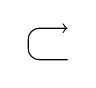
\begin{tikzpicture} [baseline, xscale=0.5, yscale=0.4] \draw[->, rounded corners] (1, 0) -- (0, 0) -- (0, 1) -- (1, 1); \end{tikzpicture}
之合成是 $\identity$: 显然 $I \mapsfrom J$ 蕴涵 $I[S^{-1}] \subset J$, 另一方面, 对任意 $[r,s] \in J$ 皆有 $[r,1] = [r,s][s,1] \in J$, 故 $r \in I$, 于是 $J \subset I[S^{-1}]$. 由此可见 $I \mapsto I[S^{-1}]$ 为满而 \eqref{eqn:ideal-preimage-localization} 为单. 然而若不限定所论的理想, 则上图按
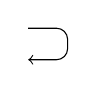
\begin{tikzpicture} [baseline, xscale=0.5, yscale=0.4] \draw[->, rounded corners] (0, 1) -- (1, 1) -- (1, 0) -- (0, 0); \end{tikzpicture}
合成未必是 $\identity$, 从以下证明可以窥见端倪.

\begin{proposition}\label{prop:localization-ideals}
	令 $S$ 为 $R$ 的乘性子集, $0 \notin S$.
	\begin{enumerate}
		\item 对任意理想 $I$, 等式 $I[S^{-1}] = R[S^{-1}]$ 成立当且仅当 $I \cap S \neq \emptyset$.
		\item 映射 $I \mapsto I[S^{-1}]$ 诱导出双射
			\[ \{I \in \Spec R : I \cap S = \emptyset \} \stackrel{1:1}{\longrightarrow} \Spec R[S^{-1}], \]
			其逆是前述之 \eqref{eqn:ideal-preimage-localization}.
		\item 上述双射保持包含关系: $I_1 \subset I_2 \iff I_1[S^{-1}] \subset I_2[S^{-1}]$.
	\end{enumerate}
\end{proposition}
\begin{proof}
	由于 $1 \in R[S^{-1}]$ 对应到形如 $[r, s]$ 并存在 $t \in S$ 使 $tr = ts \in S$ 的等价类, 立得第一条断言.

	现在设 $I \in \Spec R$, $I \cap S = \emptyset$. 则在 $R[S^{-1}]$ 中
	\[ [r_1, s_1] [r_2, s_2] \in I[S^{-1}] \iff r_1 r_2 \in I \iff \left( r_1 \in I \; \text{或} \; r_2 \in I \right), \]
	故 $I[S^{-1}]$ 为素理想. 它对 $R \to R[S^{-1}]$ 的原像等于
	\[ \{r \in R : \exists a \in I, \; s \in S, \quad [r, 1] = [a, s] \} \in \Spec R \quad \because\;\text{引理 \ref{prop:Spec-pullback}}; \]
	此集可进一步改写为 $\{ r \in R : \exists s \in S, \; rs \in I \}$, 由于 $S$ 与素理想 $I$ 不交, 此原像无非是 $I$. 配合先前的讨论, 这就证明了 $I \mapsto I[S^{-1}]$ 在素理想层面是双射. 关于包含关系的断言是显然的.
\end{proof}

前述双射又可表作
\[ \Spec R[S^{-1}] = \Spec R \smallsetminus \{I \in \Spec R : I \cap S \neq \emptyset \}. \]
若视素谱 $\Spec R$ 为某种意义下的``空间'', 不妨设想 $R \mapsto R[S^{-1}]$ 的效果是在 $\Spec R$ 中隐去与 $S$ 有交的``点'', 这就解释了局部化一词的由来. 篇幅所限, 这里还不能详细展开素谱的几何意涵.

\begin{example}\label{eg:localization-prime}
	取定 $\mathfrak{p} \in \Spec R$, 则 $S := R \smallsetminus \mathfrak{p}$ 为乘性子集. 由前述双射知 $R_\mathfrak{p} := R[S^{-1}]$ 的素理想一一对应于 $R$ 中包含于 $\mathfrak{p}$ 的素理想, 而 $\mathfrak{p}[S^{-1}] = \mathfrak{p} R_\mathfrak{p}$ 是 $R_\mathfrak{p}$ 唯一的极大理想, 尽管相应的 $\mathfrak{p} \in \Spec R$ 未必极大. 这是交换环论的常用技巧.
\end{example}

\section{间奏: Möbius 反演}\label{sec:Mobius}
Möbius 反演公式是组合学与数论中的基本工具. 之所以专辟一节讨论, 有三重目的: 一是迅速地补全我们需要的情形, 二是演示环论的一种有趣应用, 三则是说明如何从高观点梳理经典的 Möbius 反演公式, 将之阐述为偏序集中的一套计数手段. 本节将取法 \cite[\S\S 3.7--3.8]{Stan09}, 以代数工具演绎 Möbius 反演的基本理路.

\begin{definition}\index{pianxuji!局部有限}
	若非空偏序集 $(P, \leq)$ 中对任意 $x \leq y$, 子集 $[x,y] := \{ z \in P: x \leq z \leq y \}$ 皆有限, 则称 $(P,\leq)$ 为\emph{局部有限偏序集}.
\end{definition}

对于局部有限的 $(P, \leq)$, 定义环 $(I(P, \leq),+,\star)$ 如下.
\begin{compactitem}
	\item 它作为加法群由所有函数 $f: \{(x,y) \in P^2 : x \leq y \} \to \Q$ 构成, 加法为 \linebreak $(f+g)(x,y) = f(x,y) + g(x,y)$;
	\item 乘法定为 $(f \star g)(x,y) = \sum_{z: \; x \leq z \leq y} f(x,z) g(z,y)$;
	\item 乘法幺元 $\delta \in I(P, \leq)$ 为
	\[ \delta(x,y) = \begin{cases} 1, & x=y \\ 0, & x < y \end{cases} \]
	这是数学中常用的符号记法, 称为 Kronecker 的 $\delta$. \index{Kronecker 的 $\delta$}
\end{compactitem}
局部有限确保 $I(P, \leq)$ 的乘法是良定的. 环公理的验证毫无困难, 例如乘法结合律成立的缘由就和矩阵乘法情形如出一辙; 细节留给读者. 如在定义中容许函数取值在任意域 $\Bbbk$ 中, 便得到所谓 $\Bbbk$ 上的\emph{关联代数}; 域上代数的概念将在 \S\ref{sec:algebra-def} 介绍, 这里按下不表.

翻转序关系得到的 $(P, \geq)$ 依然是局部有限偏序集. 细观乘法定义可知
\begin{gather}\label{eqn:incidence-ring-op}
	I(P,\geq) = I(P, \leq)^\text{op}.
\end{gather}

\begin{lemma}\label{prop:incidence-ring-inv}
	设 $(P, \leq)$ 局部有限, 对任意 $f \in I(P, \leq)$, 以下陈述等价:
	\begin{compactitem}
		\item $f$ 有乘法左逆元,
		\item 对每个 $x \in P$ 皆有 $f(x,x) \neq 0$,
		\item $f$ 有乘法右逆元.
	\end{compactitem}
	特别地, 在环 $I(P, \leq)$ 中左可逆 $\iff$ 可逆 $\iff$ 右可逆.
\end{lemma}
\begin{proof}
	公式 $g \star f = \delta$ 展开后无非是
	\begin{align*}
		g(x,x)f(x,x) & =1, \quad x \in P \\
		g(x,y) f(y,y) & = - \sum_{x \leq z < y} g(x,z) f(z,y), \quad x,y \in P, \; x < y.
	\end{align*}
	因而此式成立蕴涵 $\forall x \; f(x,x) \neq 0$; 反之, 当 $\forall x \; f(x,x) \neq 0$ 时上式唯一地定义了 $g(x,y)$ 使得 $g \star f = \delta$. 由此可见 $f$ 左可逆等价于 $f(x,x) \neq 0$. 考虑 $(P,\geq)$ 并利用 \eqref{eqn:incidence-ring-op} 便得到右可逆的情形.
\end{proof}

对于局部有限偏序集 $(P,\leq)$, 定义
\begin{gather*}
	\zeta = \zeta_P \in I(P, \leq), \quad \forall x \leq y, \; \zeta(x,y) = 1, \\
	\mu = \mu_P \in I(P, \leq), \quad \mu := \zeta^{-1}.
\end{gather*}
此处 $\zeta$ 的可逆性由引理 \ref{prop:incidence-ring-inv} 保证. 我们也称函数 $\mu$ 为 $(P, \leq)$ 的 \emph{Möbius 函数} $\mu$. 性质 $\mu \star \zeta = \delta = \zeta \star \mu$ 展开了无非是
\begin{gather}\label{eqn:Mobius-eq}
	\sum_{z \in [x,y]} \mu(x,z) = \delta(x,y) = \sum_{z \in [x,y]} \mu(z,y).
\end{gather}
回顾引理 \ref{prop:incidence-ring-inv} 证明中的递归公式, 还能进一步导出 $\mu$ 取值在 $\Z$. 这对后续应用是要紧的.\index{Möbius 函数}\index[sym1]{mu@$\mu$}

\begin{proposition}[Möbius 反演公式 (Gian-Carlo Rota, 1964)]\label{prop:Mobius-inversion}\index{Möbius 反演 (Möbius inversion)}
	设 $(A,+)$ 为交换群. 设偏序集 $(P,\leq)$ 满足
	\[ \forall x \in P, \quad \{y \in P: y \leq x \} \;\text{有限}, \]
	则 $(P,\leq)$ 为局部有限偏序集; 并且对任意函数 $f,g: P \to A$, 有
	\[ \forall x,\quad g(x) = \sum_{y \leq x} f(y) \iff \forall x,\quad f(x) = \sum_{y \leq x} g(y) \mu(y,x). \]
\end{proposition}
\begin{proof}
	条件显然蕴涵 $(P,\leq)$ 局部有限, 且断言中的和式皆有限. 如第一式成立, 则
	\begin{align*}
	\sum_{y \leq x} g(y) \mu(y,x) & = \sum_{z \leq y \leq x} f(z) \mu(y,x) \\
	& = \sum_{z \leq x} \left( \sum_{z \leq y \leq x} \mu(y,x) \right) f(z).
	\end{align*}
	同理, 如第二式成立则
	\[ \sum_{y \leq x} f(y) = \sum_{z \leq x} \left( \sum_{z \leq y \leq x} \mu(z,y)\right) g(z). \]
	代入 $\Z$ 中的等式 \eqref{eqn:Mobius-eq} 立得断言.
\end{proof}

\begin{example}[色多项式]
	试问如何用一个有 $q$ 种颜色的色盘为一份地图上色, 使得相邻的区/县颜色相异? 下图是兰州市的例子, 我们也一并给出图论的改述.
	\begin{center}\begin{tikzpicture}
			\node (PIC) at (0,0) {\includegraphics[width=185pt]{Lanzhou.png}};
			\node (TXT) [right=2em of PIC.east, text width=150pt, align=left] {
				若用顶点对应区县, 相邻者以边相连, 那么原问题就等价于为一个有限平面图 $\Gamma$ 的每个顶点上色 ($q$ 种选择), 使得每条边的两端不同色. 如此则可探讨任意有限图的着色. 称这种着色方式为``恰当''的.
			};
			\node (NOTE) [above=0.5em of TXT.north, text width=120pt, align=left, below delimiter=|] {
				\footnotesize \textcolor{red}{$\bigstar$} 图源: \href{https://commons.wikimedia.org/wiki/File:Administrative_Division_Lanzhou.svg}{Wikimedia Commons}, 蓝线为黄河.
			};
	\end{tikzpicture}\end{center}

	记 $\Gamma$ 的所有恰当着色方式的个数为 $M_\Gamma(q)$. 为了计数, 先不管着色是否恰当, 则着色方式恰有 $q^{V(\Gamma)}$ 种, 其中 $V(\Gamma)$ 为顶点或者说区县的个数. 我们称 $\Gamma'$ 是 $\Gamma$ 的子地图, 如果 $\Gamma'$ 是从 $\Gamma$ 合并若干行政区划得到的, 或从图论角度看就是缩并, 记为 $\Gamma' \leq \Gamma$. 如是则使 $\Gamma$ 的全体子地图对 $\leq$ 构成有限偏序集. 于是看出
	\[ q^{V(\Gamma)} = \sum_{\Gamma' \leq \Gamma} M_{\Gamma'}(q); \]
	诚然, 对任何一种地图着色, 总能合并相邻的同色区县使之变为恰当的. 现在应用命题 \ref{prop:Mobius-inversion} 导出
	\[ M_\Gamma(q) = \sum_{\Gamma' \leq \Gamma} q^{V(\Gamma')} \mu(\Gamma', \Gamma).  \]
	视 $q$ 为变元, 则整系数多项式 $M_\Gamma(q)$ 给出图 $\Gamma$ 的一个代数不变量, 称为 $\Gamma$ 的色多项式, 这是 Birkhoff 研究四色问题时引入的. 在统计物理学中, $M_\Gamma(q)$ 对应于反铁磁 $q$-态 Potts 模型的配分函数在零温极限的情形; 见 \cite{Sok05}.
\end{example}

下一步是推导经典的 Möbius 反演, 仍需几道工序.
\begin{lemma}\label{prop:Mobius-prod}
	设 $(P_1, \leq), \ldots, (P_n, \leq)$ 为局部有限偏序集. 赋予积集 $P := \prod_{i=1}^n P_i$ 序结构 $(x_i)_{i=1}^n \leq (y_i)_{i=1}^n \iff \forall i\; x_i \leq y_i$, 则 $(P, \leq)$ 依然是局部有限偏序集, 其 Möbius 函数为
	\[ \mu_P\left( x, y \right) = \prod_{i=1}^n \mu_{P_i}(x_i, y_i), \quad x=(x_i)_i, \; y=(y_i)_i \in P \]
\end{lemma}
\begin{proof}
	极易看出 $(P, \leq)$ 是局部有限偏序集. 剩下工作是对如上定义的 $\mu_P$ 验证 \eqref{eqn:Mobius-eq}, 这可以归结为 $P$ 上的求和公式
	\begin{equation*}
		\sum_{\substack{z = (z_i)_i \in P \\ x \leq z \leq y}} = \sum_{x_1 \leq z_1 \leq y_1} \cdots \sum_{x_n \leq z_n \leq y_n}.
	\end{equation*}
\end{proof}

尚需一个毫不困难的推广. 考虑一族局部有限的偏序集 $(P_i, \leq)_{i \in I}$. 假定对``几乎所有的''下标 $i$ (确切地说, 至多有限个下标除外), 我们取定了元素 $\mathring{x}_i \in P_i$. 定义所谓\emph{受限积} $P := \Resprod_i P_i$ 为
\[ \left\{ (x_i)_i \in \prod_{i \in I} P_i : \text{对几乎所有 $i$, 有}\; x_i = \mathring{x}_i  \right\} \]
此处 $\Resprod_i P_i$ 继承 $\prod_i P_i$ 的积偏序: $(x_i)_i \leq (y_i)_i \iff \forall i\; x_i \leq y_i$. 那么 $(P, \leq)$ 仍然局部有限, 而且 Möbius 函数的表法照旧
\[ \mu_P\left( x, y \right) = \prod_i \mu_{P_i}(x_i, y_i) \]
对几乎所有 $i$ 都有 $x_i = y_i = \mathring{x}_i$ 而 $\mu_{P_i}(\mathring{x}_i, \mathring{x}_i)=1$, 乘积因之有限. 欲证上式仅须对每个 $x \leq y$ 验证 \eqref{eqn:Mobius-eq}, 然而该式中仅涉及使得 $x_i, y_i \neq \mathring{x}_i$ 的有限多个下标 $i$, 问题立刻化约到有限积的情形. 现在可以阐述经典的 Möbius 反演公式.

\begin{example}
	考虑全序集 $(\Z_{\geq 0}, \leq)$, 它当然使得 $\{y: y \leq x\}$ 对每个 $x$ 皆为有限集. 取
	\[ \mu(n,m) := \begin{cases} 1, & n-m = 0 \\ -1, & n-m = -1, \\ 0, & \text{其它情形}. \end{cases} \]
	不待计算立见 \eqref{eqn:Mobius-eq} 成立. 此即所求的 Möbius 函数. 在此特例下, 请读者将命题 \ref{prop:Mobius-inversion} 的反演公式翻译为一望可知的计数原理.
\end{example}

\begin{example}[A.\ F.\ Möbius, 1832]\label{eg:Mobius-classical}
	现在赋予 $\Z_{\geq 1}$ 整除偏序: 定义 $n \prec m \iff n \mid m$; 同样地, $\{y : y \prec x \}$ 对每个 $x$ 都有限, 因为每个正整数仅有有限多个因子. 正整数的唯一分解给出偏序集的同构 (即保序双射):
	\begin{align*}
		\Resprod_{p: \text{素数}} (\Z_{\geq 0}, \leq) & \longrightiso (\Z_{\geq 1}, \prec) \\
		(n_p)_p & \longmapsto \prod_{p: \text{素数}} p^{n_p},
	\end{align*}
	左端实际是之前解释过的受限积, 取 $\mathring{x}_p = 0$. 因此 $\prod_p p^{n_p}$ 有限, 映射是良定的. 根据引理 \ref{prop:Mobius-prod} 的受限积版本, $(\Z_{\geq 1}, \prec)$ 的 Möbius 函数 $\mu$ 表作
	\begin{align*}
		\mu\left( \prod_p p^{n_p}, \prod_p p^{m_p} \right) & = \prod_{p: \text{素数}} \mu_{(\Z_{\geq 0}, \leq)}(n_p, m_p) \\
		& =\begin{cases}
			\prod_{\substack{p: \text{素数}}} (-1)^{n_p - m_p}, & \forall p \quad n_p-m_p \geq -1 \\
			0, & \exists p\quad n_p - m_p < -1.
	\end{cases}\end{align*}
	记 $\mu(n) := \mu(1,n)$, 则 $\mu(d,n) = \mu(n/d)$, 而上式给出直截了当的描述
	\[ \mu(n) = \begin{cases}
		(-1)^{(n\; \text{的素因子个数})}, & n\; \text{无平方因子} \neq 1, \\
		0, & \text{其它情形}.
	\end{cases} \]
	对于交换群 $(A,+)$ 及任意函数 $f, g: \Z_{\geq 1} \to A$, 命题 \ref{prop:Mobius-inversion} 化作
	\[ \forall n,\; g(n) = \sum_{d \mid n} f(d) \iff \forall n,\; f(n) = \sum_{d \mid n} g(d) \mu\left( \frac{n}{d} \right). \]
	
	此即熟知的 Möbius 反演公式, 实践中又分为
	\begin{inparaenum}[(a)]
		\item 加性情形: $A$ 取为 $\Z$, $\CC$ 等加法群, 以及
		\item 乘性情形: $A$ 取为 $\Q^\times$ 或非零有理多项式 $\Q(X)^\times$ 等乘法群.
	\end{inparaenum}
	但理论框架并无二致.
\end{example}

现在来考虑一个初等应用. 对于任意 $n \in \Z_{\geq 1}$, 熟知的 Euler 函数 $\varphi(n) := |(\Z/n\Z)^\times|$ 无非是计算所有 $\leq n$ 而与 $n$ 互素的正整数个数. 以下等式恒成立:
\begin{equation}\label{eqn:Euler-phi-sum}\begin{gathered}
	\sum_{d \mid n} \varphi(d) = n, \\
	\sum_{d \mid n} d \mu\left( \frac{n}{d} \right) = \varphi(n).
\end{gathered}\end{equation}
第一式的一种解释如下: 将 $n$ 个有理数 $\frac{1}{n}, \ldots, \frac{n}{n}$ 全化作最简分数, 则 $\varphi(d)$ 正好是其中分母化为 $d$ 的元素个数; 应用 Möbius 反演立得第二式. 这些都是初等数论中熟知的性质.

\section{环的极限与完备化}\label{sec:ring-limits}
本节中出现的 $I$ 皆为非空集或非空范畴. 我们将按照直积, $\varprojlim$ 和 $\varinjlim$ 的顺序解说, 顺带引入点集拓扑的语言来讨论完备化.

\begin{definition}\label{def:ring-direct-product}
	设 $\{R_i : i \in I\}$ 为一族环. 其直积 $\prod_{i \in I} R_i$ 在加法群的层次与定义 \ref{def:monoid-times} 相同, 我们在 $\prod_{i \in I} R_i$ 上定义乘法运算为
	\[ (r_i)_{i \in I} \cdot (s_i)_{i \in I} = (r_i \cdot s_i)_{i \in I}. \]
	换言之, $\prod_{i \in I} R_i$ 同时是乘法幺半群的直积, 其幺元是 $(1_{R_i})_{i \in I}$. 易证 $\prod_{i \in I} R_i$ 满足环的公理.
\end{definition}

对每个 $j \in I$, 投影映射 $(r_i)_{i \in I} \mapsto r_j$ 是 $\prod_{i \in I} R_i$ 到 $R_j$ 的环同态. 环直积及其投影同态在环范畴中也满足泛性质 (对照引理 \ref{prop:product-monoid-univ-prop}), 证明与幺半群情形相同, 此处略去.

\begin{theorem}[中国剩余定理]\label{prop:CRT}\index{zhongguoshengyudingli@中国剩余定理 (Chinese Remainder Theorem)}
	设 $R$ 为环, $I_1, \ldots I_n$ 为一族理想. 假设对每个 $i \neq j$ 皆有 $I_i + I_j = R$, 则环同态
	\begin{align*}
		\varphi: R & \longrightarrow \prod_{i=1}^n R/I_i, \\
		r & \longmapsto \left( r \bmod I_i \right)_{i=1}^n
	\end{align*}
	诱导出环同构 $R \big/ (\bigcap_{i=1}^n I_i) \rightiso \prod_{i=1}^n R/I_i$.
\end{theorem}
连带地, $\varphi$ 也诱导群同构 $\left( R \big/ (\bigcap_{i=1}^n I_i)\right)^\times \rightiso \prod_{i=1}^n \left(R/I_i\right)^\times$.
\begin{proof}
	显然 $\Ker(\varphi) = \bigcap_{i=1}^n I_i$, 仅须证明 $\varphi$ 是满的. 取定 $1 \leq i \leq n$, 对每个 $j \neq i$ 存在 $r_j \in I_i$ 和 $s_j \in I_j$ 使得 $r_j + s_j = 1$. 以下的连乘积 $\prod_j$ 约定为按 $j=1,2,\ldots$ 循序相乘: 展开 $1 = \prod_{j \neq i} (r_j + s_j)$ 并分离 $s := \prod_j s_j \in \prod_{j \neq i} I_j$ 与其余诸项之和 $r \in I_i$, 遂得
	\[ 1 = r + s \in I_i + \prod_{j \neq i} I_j. \]
	因此 $y_i := s$ 在 $R/I_j$ ($j \neq i$) 中的像是 $0$, 在 $R/I_i$ 中的像是 $1$. 由于对任意 $x_1, \ldots, x_n \in R$ 有
	\[ \varphi(x_1 y_1 + \cdots + x_n y_n) = (x_i \bmod I_i)_{i=1}^n, \]
	故 $\varphi$ 确为满射.
\end{proof}

现于定理中取 $R=\Z$, $I_i = a_i \Z$, 其中 $a_i \geq 1$; 如置 $a$ 为 $a_1, \ldots, a_n$ 的最小公倍数, 则 $\bigcap_{i=1}^n I_i = a\Z$. 定理的条件相当于 $a_1, \ldots, a_n$ 两两互素, 而结论是说 $\Z/a\Z \rightiso \prod_{i=1}^n \Z/a_i\Z$. 这是中国剩余定理在初等数论中的面貌.

今将证明环范畴 $\cate{Ring}$ \index[sym1]{Ring@$\cate{Ring}$} 中存在非空的 $\varprojlim$. 下面沿用 \S\ref{sec:limits} 的符号, 考虑函子 $\beta: I^\text{op} \to \cate{Ring}$, 其中 $I$ 是小范畴 (见约定 \ref{con:U-small}). 为了符号方便, 不妨就假定 $I$ 实际是一个小的非空偏序集 $(I, \leq)$, 而 $\beta$ 对应到环族 $\{R_i = \beta(i) \}_{i \in I}$ 及同态族 $\{\varphi_{ij} = \beta(j \to i): R_i \to R_j \}_{i \geq j}$, 后者须满足相容条件
\[ i \geq j \geq k \implies \varphi_{jk} \varphi_{ij} = \varphi_{ik}: R_i \to R_k. \]

下面构造极限 $\varprojlim \alpha = \varprojlim_{i \in I} R_i$, 其手法与群的情形 \S\ref{sec:group-limit} 是一贯的.

\begin{proposition}
	定义 $\prod_{i \in I} R_i$ 的子环
	\[ \varprojlim_{i \in I} R_i := \left\{ (r_i)_{i \in I} \in \prod_{i \in I} R_i : \; \forall i \geq j,\; \varphi_{ij}(r_i) = r_j \right\}. \]
	则 $\varprojlim_{i \in I} R_i$ 连同投影同态族 $\left( p_j: \varprojlim_{i \in I} R_i \to R_j \right)_{j \in I}$ 满足如下泛性质: 对任意环 $S$ 及同态族 $(q_j: S \to R_j)_{j \in I}$, 若图表
	\[ \begin{tikzcd}
		S \arrow[r, "q_i"] \arrow[rd, "q_j"'] & R_i \arrow[d, "\varphi_{ij}"] \\
		&  R_j
	\end{tikzcd} \]
	对 $I$ 中每个 $i \geq j$ 皆交换, 则存在唯一环同态 $\varphi: S \to \varprojlim_{i \in I} R_i$ 使下图对每个 $j \in I$ 皆交换:
	\[ \begin{tikzcd}
		S \arrow[r, "q_j"] \arrow[d, "{\exists! \, \varphi}"'] & R_j \\
		\varprojlim_{i \in I} R_i \arrow[ru, "p_j"'] &
	\end{tikzcd} \]
\end{proposition}
\begin{proof}
	由于每个 $\varphi_{ij}$ 都是环同态, 易见 $\varprojlim_i R_i$ 为 $\prod_{i \in I} R_i$ 的子环. 图表交换相当于说对每个 $s \in S$ 皆有 $\varphi(s) = (q_i(s))_{i \in I}$, 后者落在 $\varprojlim_i R_i$ 中当且仅当 $(S, q_i)$ 满足命题中的交换性条件. 这就唯一给出了 $\varphi$.
\end{proof}

对于一般的小范畴 $I$, 极限 $\varprojlim \beta \subset \prod_{i \in \Obj(I)} \beta(i)$ 的构造方法完全类似. 现在转向其特例完备化, 假设 $(I, \leq)$ 为滤过偏序集 (定义 \ref{def:filtrant-poset}).

\begin{definition}[环的完备化]\label{def:ring-completion}\index{wanbeihua}
	设 $R$ 为环, $(\mathfrak{a}_i)_{i \in I}$ 为一族 $R$ 的双边真理想, 使得 $i \geq j$ 蕴涵 $\mathfrak{a}_i \subset \mathfrak{a}_j$, 从而导出商映射 $\varphi_{ij}: R/\mathfrak{a}_i \to R/\mathfrak{a}_j$. 相应的极限 $\varprojlim_{i \in I} R/\mathfrak{a}_i$ 称作 $R$ 对 $(\mathfrak{a}_i)_{i \in I}$ 的\emph{完备化}.
\end{definition}
从商同态族 $R \to R/\mathfrak{a}_i$ 导出自然的环同态 $\iota: R \to \varprojlim_i R/\mathfrak{a}_i$, 其核是 $\bigcap_i \mathfrak{a}_i$; 以 $R/\Ker(\iota)$ 代 $R$, 总能化约到 $\Ker(\iota)=\{0\}$ 的情形, 以下不妨如是假设.

令 $\mathfrak{A}_j$ 表 $\varprojlim_i R/\mathfrak{a}_i \to R/\mathfrak{a}_j$ 的核, 即
\[ \mathfrak{A}_j = \left\{ (r_i)_{i \in I} \in \varprojlim_i R/\mathfrak{a}_i : \; i \leq j \implies r_i=0 \right\}. \]
兹引进\emph{拓扑环}的概念: \index{tuopuhuan@拓扑环, 拓扑域, 拓扑模} 这意谓一个环兼有拓扑空间结构, 而环的加法, 取负和乘法皆连续; 特别地, 拓扑环对加法构成拓扑交换群. 现在赋予每个 $R_i := R/\mathfrak{a}_i$ 离散拓扑, 则 $\varprojlim_{i \in I} R/\mathfrak{a}_i$ 无非是对加法群 $R$ 及 $\{\mathfrak{a}_i\}_{i \in I}$ 作定义 \ref{def:group-completion} 的完备化. 因而 $(\varprojlim_i R_i, +)$ 成为完备 Hausdorff 拓扑群, 理想族 $\{\mathfrak{A}_i\}_{i \in I}$ 给出 $0$ 处的邻域基. 进一步, $\varprojlim_i R_i$ 成拓扑环: 乘法连续性是下述性质的直接推论
\[ (j,k \geq i) \implies \mathfrak{A}_j \cdot \mathfrak{A}_k \subset \mathfrak{A}_i. \]
若每个 $R/\mathfrak{a}_i$ 皆为有限环, 则从引理 \ref{prop:completion-compactness} 知 $\varprojlim_i R/\mathfrak{a}_i$ 是紧的.

\begin{remark}\label{rem:ring-completion} \index{a-jintuopu@$\mathfrak{a}$-进拓扑}
	令 $\hat{R} := \varprojlim_i R/\mathfrak{a}_i$. 就拓扑观点看, 这里的构造相当于令 $(\mathfrak{a}_i)_{i \in I}$ 为 $0 \in R$ 的一组邻域基, 使 $R$ 成 Hausdorff 拓扑环 (见 \eqref{eqn:top-group-Hausdorff}), 再仿照 \S\ref{sec:group-limit} 作环 $R$ 的完备化 $\hat{R}$. 一如群的情形, 环的完备化意谓一个连续环同态 $\iota: R \to \hat{R}$, 由以下性质刻画 (精确到唯一同构):
	\begin{compactenum}[\bfseries {CO}.1]
		\item $\iota: R \to \iota(R)$ 为同胚,
		\item $\iota$ 的像稠密,
		\item $\hat{R}$ 是完备的 Hausdorff 拓扑环.
	\end{compactenum}
	实践中常取定一个双边理想 $\mathfrak{a}$, 考虑全序集 $I = (\Z_{\geq 0}, \leq)$ 和 $\mathfrak{a}_i = \mathfrak{a}^{i+1}$; 此时 $R$ 上的拓扑称为 $\mathfrak{a}$-进拓扑. 如果存在 $\mathfrak{a}$ 使得 $R$ 带 $\mathfrak{a}$-进拓扑, 我们则称 $R$ 带有进制拓扑, 这是一类常见的拓扑环. 留意到 $\mathfrak{a}$ 的选取并不唯一: 读者可以验证对任意 $k \in \Z_{\geq 1}$, 由 $\mathfrak{a}^k$ 和 $\mathfrak{a}$ 确定的进制拓扑是一样的. 
\end{remark}

\begin{example}\label{eg:Z_p}
	考虑环 $R = \Z$ 及其理想族 $\mathfrak{a}_i := p^{i+1} \Z$, 其中 $p$ 是取定的素数. 相应的完备化 $\Z_p$ 称为 $p$-进整数环, 它是 $\Z$ 对其 $p\Z$-进拓扑 (今后简称 $p$-进拓扑) 的完备化.
\end{example}

\begin{example}\label{eg:Prüfer}
	取集合 $I := \Z_{> 1}$, 并以整除性定义滤过偏序: $N \prec N' \iff N \mid N'$, 此时有商同态 $\Z/N'\Z \to \Z/N\Z$. 相应的完备化 $\hat{\Z} := \varprojlim_N \Z/N\Z$ 称作 Prüfer 环. 事实上 $\hat{\Z} \simeq \prod_p \Z_p$, 其中 $p$ 取遍素数. 缘由如下: $N$ 有唯一的素因子分解 $N = \prod_p p^{v_p(N)}$, 对任意 $N \prec N'$ 皆有交换图表
	\[ \begin{tikzcd}
		\prod_p (\Z/p^{v_p(N')}\Z ) \arrow[twoheadrightarrow, d] \arrow[r, "\sim"] & \Z/N'\Z \arrow[twoheadrightarrow, d] \\
		\prod_p (\Z/p^{v_p(N)}\Z ) \arrow[r, "\sim"'] & \Z/N\Z
	\end{tikzcd} \]
	其中横向同构来自中国剩余定理, 纵向是商同态. 左右比较完备化得 $\prod_p \Z_p \rightiso \hat{\Z}$.
\end{example}

环 $\Z_p$ 是完备化的典型. 鉴于其应用之广, 以下将进一步探讨 $\Z_p$ 的性质, 同时演示交换环论中的一些基本技巧. 首先, 观察到 $\varprojlim$ 的构造蕴涵
\begin{align*}
	p^{n+1} \Z_p & = \left\{ (x_i)_{i \geq 0} : x_i \in p^{n+1} \cdot \Z/p^{i+1}\Z \right\} \\
	& = \left\{ (x_i)_{i \geq 0} : i \leq n \implies x_i=0 \right\} = \Ker\left[ \Z_p \stackrel{p_n}{\twoheadrightarrow} \Z/p^{n+1}\Z \right].
\end{align*}
从而 $\Z_p/p^{n+1}\Z_p \rightiso \Z/p^{n+1}\Z$. 这也蕴涵 $p\Z_p$ 是极大理想. 此外留意到 $p$ 在 $\Z_p$ 中非零因子: 如果 $(x_i)_i \neq 0$, 取 $n$ 使得 $x_{n-1} \neq 0$, 则必有 $x_n \notin p^n \Z/p^{n+1}\Z$, 从而 $px_n \neq 0$.

对任意 $x = \left( x_i \in \Z/p^{i+1}\Z \right)_{i \geq 0} \in \Z_p$, 由以上观察可以定义
\[ v_p(x) := \sup\{n: x \in p^n\Z_p \} = \inf\{n : x_n \neq 0\}. \]
函数 $v_p: \Z_p  \to \Z_{\geq 0} \sqcup \{\infty\}$ 称为 $p$-进赋值.

\begin{proposition}\label{prop:p-adic}\index[sym1]{Z_p}
	对任意素数 $p$, 以下性质成立.
	\begin{enumerate}
		\item $\Z_p$ 是整环, 而且 $v_p(x) = \infty \iff x=0$.
		\item 对任意 $x,y \in \Z_p$
			\begin{align*}
				v_p(xy) & = v_p(x) + v_p(y), \\
				v_p(x+y) & \geq \min\{v_p(x), v_p(y)\}, \quad \text{(强三角不等式)}.
			\end{align*}
		\item 元素 $x \in \Z_p$ 可逆当且仅当 $v_p(x)=0$.
		\item $\Z_p$ 是主理想环, 其非零理想皆为 $p^n \Z_p = \{x \in \Z_p: v_p(x) \geq n \}$ 的形式.
  \end{enumerate}
\end{proposition}
\begin{proof}
	记 $W := \Z_p$. 之后的论证仅需要定义 $v_p(x) = \sup\{n: x \in p^n W\}$ 和业已经观察过的性质:
	\begin{inparaenum}[(a)]
		\item $W \rightiso \varprojlim_{n \geq 0} W/p^{n+1}W$;
		\item $p$ 在 $W$ 中不是零因子;
		\item $W/pW$ 是域.
	\end{inparaenum}

	首先, $v_p(x)=\infty$ 等价于 $x \in \bigcap_{n \geq 0} p^{n+1}W$, 然而 (a) 蕴涵此时 $x=0$. 接着证明 $W$ 为整环: 若 $x,y \in W$ 皆非零, 由前一步可假设 $x=p^{v_p(x)} x'$, $y=p^{v_p(y)} y'$ 满足于 $x',y' \notin pW$, 再由 (b) 知问题化为证 $x'y' \neq 0$. 然而 $W/pW$ 是域故 $x'y' \notin pW$, 特别地 $x'y' \neq 0$.

	下面证明 $v_p$ 的两条性质. 同样置 $x = p^{v_p(x)} x'$ 和 $y = p^{v_p(y)} y'$. 不妨设 $v_p(x) \geq v_p(y)$, 则 $x+y \in p^{v_p(y)}W$ 故 $v_p(x+y) \geq \min\{ v_p(x), v_p(y)\}$. 又从 $x'y' \notin pW$ 可导出 $v_p(xy) = v_p(x) + v_p(y)$.

	令 $x \in W^\times$, 考虑其模 $pW$ 的像可知 $v_p(x) = 0$. 相反地, 假设 $x \in W \smallsetminus pW$, 由 (c) 知存在 $a \in W$ 使得 $ax \equiv 1 \pmod{pW}$. 因此不妨假设 $x \equiv 1 \pmod{pW}$. 置 $x = 1-t$, $v_p(t) \geq 1$. 在 Hausdorff 拓扑环 $W$ 中有等式
	\[ x(1 + t + \cdots + t^N) = (1 - t)(1 + t + \cdots + t^N) = 1 - t^{N+1}. \]
	当 $N \to \infty$ 时右式趋近于 $1$. 如能证明 $y_N := 1+ t +\cdots + t^N$ 亦收敛, 则其极限给出 $x^{-1}$. 为此, 仅需观察到对于 $N' \geq N$, 和式 $y_{N'}$ 中 $t^N$ 以后的项不影响它模 $p^N W$ 的类.

	最后证明关于理想的断言. 假设 $I$ 是 $W$ 中的非零理想. 定义 $n := \min\{v_p(x) : x \in I\}$, 于是 $I \subset p^n W$. 取非零元 $x = p^n y \in I$ 满足 $v_p(x)=n$, 于是 $y$ 必可逆, 从而 $p^n W = xW \subset I$. 明所欲证.
\end{proof}

环 $\Z_p$ 对乘性子集 $\{1,p,p^2,\ldots\}$ 的局部化 $\Z_p[\frac{1}{p}] =: \Q_p$ 称为 \emph{$p$-进数域}. 由以上对可逆元的刻画知 $\Q_p = \text{Frac}(\Z_p)$, 其非零元可以唯一地表作 $p^a t$ 的形式, 其中 $t \in \Z_p^\times$ 而 $a \in \Z$. 同时赋值 $v_p$ 在 $\Q_p$ 上有自然延拓: $v_p(p^a t) = a$; 请读者验证命题 \ref{prop:p-adic} 的不等式在 $\Q_p$ 上仍旧成立. 另一方面, $\Q_p$ 也可以视为域 $\Q$ 对赋值 $v_p\big|_\Q$ 的完备化, 一步到位地构造, 这点将在 \S\ref{sec:valued-field} 作细致讨论.

下面转向 $\varinjlim$ 的研究. 考虑小范畴 $I$ 及函子 $\alpha: I \to \cate{Ring}$. 我们即将为滤过的 $I$ 定义极限 $\varinjlim \alpha$ (定义 \ref{def:filtrant-cat}). 应用中 $I$ 往往是滤过偏序集, 不过为突出滤过条件的作用, 我们将不厌其烦地处理一般情形. 且先回忆对 $I$ 中的每个态射 $f: i \to j$, 都有相应的环同态 $\alpha(f): \alpha(i) \to \alpha(j)$.

假设 $I$ 滤过. 在例 \ref{eg:set-limits} 中, 我们业已在 $\bigsqcup_{i \in \Obj(I)} \alpha(i)$ 上以 \eqref{eqn:filtrant-equiv} 定义了等价关系 $\sim$, 从而将 $\cate{Set}$ 中的 $\varinjlim \alpha$ 实现为相应的商集 $\bigsqcup_{i \in \Obj(I)} \alpha(i) \big/ \sim$; 对每个 $j \in \Obj(I)$ 皆有映射
\[ \iota_j: \alpha(j) \to \bigsqcup_{i \in \Obj(I)} \alpha(i) \xrightarrow{\text{商映射}} \varinjlim \alpha. \]

今将往证商集 $\varinjlim \alpha$ 上具有唯一的环结构使得对每个 $f: j \to j'$,
\begin{equation}\label{eqn:filtrant-lim-ring} \begin{tikzcd}[row sep=small]
	\alpha(j) \arrow[rd, "\iota_j"'] \arrow[rr, "\alpha(f)"] & & \alpha(j') \arrow[ld, "{\iota_{j'}}"] \\
	& \varinjlim \alpha &
\end{tikzcd}\end{equation}
皆是 $\cate{Ring}$ 中的交换图表.

我们沿用构造集合的滤过极限时的符号. 定义 $\varinjlim \alpha$ 的环结构如下: 对其中任两个等价类 $[r_i]$, $[r'_j]$, 按滤过范畴定义总能找到从 $i,j$ 到某个 $k \in \Obj(I)$ 的箭头以及 $r_k, r'_k \in \alpha(k)$ 使得 $[r_i] = [r_k]$ 且 $[r'_j] = [r'_k]$. 在 \eqref{eqn:filtrant-lim-ring} 中取 $f = \identity: k \to k$ 可知 $[r_i][r'_j]$ 的定义只能是 $[r_k r'_k]$. 同样手法可以证明此乘法良定, 并给出环结构 (幺元为 $1 \in \alpha(i)$ 的等价类, $i$ 任取) 使得 \eqref{eqn:filtrant-lim-ring} 恒交换: 在比较种种不同选取给出的乘法时, 我们总是可以在范畴 $I$ 中走得足够``深''以消除所有不确定性, 这是定义 \ref{def:filtrant-cat} 的要旨. 这就验证了断言.

\begin{proposition}\label{prop:ring-filtrant-limit}
	对滤过小范畴 $I$ 和 $\alpha: I \to \cate{Ring}$ 如上, 环 $\varinjlim \alpha$ 连同同态族 $\iota_j: \alpha(j) \to \varinjlim \alpha$ 构成范畴 $\cate{Ring}$ 中的 $\varinjlim \alpha$.
\end{proposition}
\begin{proof}
	若忘掉环结构, $\varinjlim \alpha$ 作为集合是 $\alpha(i)$ 在 $\cate{Set}$ 中的极限. 因而对任意环 $R$ 及同态族 $\left( \iota'_j: \alpha(j) \to R \right)_{j \in \Obj(I)}$ 使得图表
	\[ \begin{tikzcd}[row sep=tiny]
		\alpha(i) \arrow[dd, "\alpha(f)"'] \arrow[rd, "\iota'_i"] & \\
		& R \\
		\alpha(j) \arrow[ru, "\iota'_j"'] &
		\end{tikzcd} \qquad (f: i \to j) \]
	恒交换者, 存在唯一的集合映射 $\varphi: \varinjlim \alpha \to R$ 使得
	\[ \begin{tikzcd}
		\alpha(i) \arrow[r, "\iota_i"] \arrow[rd, "\iota'_i"'] & \varinjlim \alpha \arrow[d, "\varphi"] \\
		& R
	\end{tikzcd} \qquad i \in \Obj(I) \]
	恒交换. 事实上 $\varphi([r_i]) = \iota'_i(r_i)$, 需要证明的是 $\varphi$ 为环同态. 论证与先前类似: 应用滤过范畴的条件, 再配合环同态族 $\iota'_j: \alpha(j) \to R$ 的性质即可, 细节留予读者.
\end{proof}

以上皆假设 $I$ 非空, 现在补全 $I$ 是空范畴的情形. 注意到空 $\varinjlim$ 无非是范畴中的始对象. 从 \eqref{eqn:ring-struct-morphism} 及随后的讨论, 立得以下简单而重要的结果.
\begin{proposition}
	整数环 $\Z$ 是环范畴 $\cate{Ring}$ 的始对象.
\end{proposition}

读者可能要问: 环范畴里是否总有一般的小 $\varinjlim$? 由于本章只论非零含幺环, 答案是否定的: 以下例子说明一对同态 $f,g: R \to S$ 的余等化子未必存在. 考虑多项式环 $R = \CC[X]$ 和 $S = \CC$, 取同态 $f: P \mapsto P(0)$ 和 $g: P \mapsto P(1)$, 其中 $P \in \CC[X]$. 若有环同态 $h: S \to T$ 满足 $hf=hg$, 取 $P(X)=-X$ 则有 $h(1) = h(P(0)-P(1)) = 0$, 这与 $h(1)=1$ 矛盾.

\section{从幺半群环到多项式环}\label{sec:polynomial-ring}
读者对有理系数多项式环 $\Q[X] = \left\{ a_0 + a_1 X + \cdots + a_n X^n : n \geq 0, \; a_i \in \Q \right\}$ 理应是熟悉的, 它作为 $\Q$-向量空间以 $\{ X^i : i \geq 0 \}$ 为基, 其间的乘法不外是幺半群 $(\Z_{\geq 0}, +)$ 上加法的改述. 若代之以一般的幺半群便得到如下推广. 以下固定环 $R$, 考察以其元素为系数的多项式.

\begin{definition}\label{def:monoidal-ring}\index{yaobanqunhuan@幺半群环}\index[sym1]{$R[M]$}
	令 $M$ 为幺半群. \emph{幺半群环} $R[M]$ 定义如下: 其元素是积集 $R^M$ 中形如 $(r_m)_{m \in M}$ 的列, 至多仅有限多项非零; 惯常将 $(r_m)_{m \in M}$ 形式地写作 $R$ 上的有限线性组合
	\[ f = \sum_{m \in M} r_m m, \]
	这里的 $r_m$ 称为 $m$ 在 $f$ 中的系数. 分别定义 $R[M]$ 的加法和乘法为
	\begin{align*}
		\left( \sum_m r_m m \right) + \left( \sum_m s_m m \right) & = \sum_m (r_m + s_m) m, \\
		\left( \sum_m r_m m \right) \cdot \left( \sum_m s_m m \right) & = \sum_m \left( \sum_{\substack{x, y \in M \\ xy=m}} r_x s_y \right) m,
	\end{align*}
	易见其中每个和都仅有有限个非零项, 故运算良定.
\end{definition}

不难验证 $R[M]$ 满足环的公理, 其零元是 $0 = \sum_m 0 \cdot m$, 幺元是 $1 = 1_R \cdot 1_M$: 这里的 $1_R$, $1_M$ 分别表 $R$ 和 $M$ 的幺元. 事实上 $R[M]$ 的乘法运算是由 $(rm) \cdot (r'm') = rr' (mm')$ 和分配律所唯一确定的 ($r,r' \in R$, $m, m' \in M$). 乘法结合律仅须对形如 $rm$ 的项验证即可.

注意到幺半群环带有自然的同态
\[\begin{tikzcd}[row sep=tiny]
	M \arrow[r, "\text{幺半群}"] & (R[M], \cdot) \\
	m \arrow[mapsto, r] \arrow[phantom, u, sloped, "\in" description] & 1 \cdot m \arrow[phantom, u, sloped, "\in" description]
\end{tikzcd} \quad
\begin{tikzcd}[row sep=tiny]
	R \arrow[r, "\text{环}"] & R[M] \\
	r \arrow[mapsto, r] \arrow[phantom, u, sloped, "\in" description] & r \cdot 1. \arrow[phantom, u, sloped, "\in" description]
\end{tikzcd}\]
两者皆单, 而且其像在 $R[M]$ 中对乘法互相交换, 即 $(r \cdot 1)(1 \cdot m) = (1 \cdot m)(r \cdot 1)$ (尽管 $R$, $M$ 各自都未必交换). 这为 $R[M]$ 的构造提供了一个泛性质的解释.

\begin{proposition}\label{prop:monoid-ring-universal}
	幺半群环由下述泛性质刻画: 对任意环 $S$, 幺半群同态 $f: M \to (S, \cdot)$ 及环同态 $g: R \to S$, 若 $f$ 和 $g$ 的像对 $S$ 的乘法互相交换, 则存在唯一的环同态 $\varphi: R[M] \to S$, 使得 $f$ 和 $g$ 分别等于 $M \to R[M]$ 和 $R \to R[M]$ 合成上 $\varphi$.
\end{proposition}
\begin{proof}
	唯一的取法是 $\varphi(rm) = g(r)f(m)$. 细节留给读者.
\end{proof}

倘若读者愿提前调用 \S\ref{sec:algebra-def} 的语汇, 特别是命题 \ref{prop:algebra-as-homomorphism}, 那么当 $R$ 交换时上述同态 $R \hookrightarrow R[M]$ 赋予 $R[M]$ 一个 $R$-代数的结构; 职是之故, $R[M]$ 也称为交换环 $R$ 上的\emph{幺半群代数}.

\begin{definition}\label{def:group-ring}\index{qunhuan@群环, 群代数 (group ring, group algebra)}
	当 $M$ 为群时, 环 $R[M]$ 称为 $M$ 在 $R$ 上的\emph{群环}. 当 $R$ 交换时也称之为 $R$ 上的\emph{群代数}.
\end{definition}

群环是表示理论的基本语言. 这里先回到本节开头的楔子, 同时也是环论中最基本的构造之一: 多项式环.
\begin{definition}[多项式环]\index{duoxiangshihuan@多项式环 (polynomial ring)} \index[sym1]{$R[X,\ldots]$}
	对集合 $\mathcal{X}$ 取 $(\mathbf{M}(\mathcal{X}), \cdot)$ 为 $\mathcal{X}$ 上的自由交换幺半群 (定义 \ref{def:free-comm-monoid}, 注意: 此处改用乘法符号), 则 $R[\mathcal{X}] := R[\mathbf{M}(\mathcal{X})]$ 称为 $R$ 上以 $\mathcal{X}$ 为变元集的多项式环, 它带有自然映射 $\mathcal{X} \to R[\mathcal{X}]$. 当 $\mathcal{X} = \{X, Y, \ldots\}$ 时也写作 $R[\mathcal{X}] = R[X, Y, \ldots]$.
\end{definition}
当 $R$ 交换时, 也称 $R[\mathcal{X}]$ 是以 $\mathcal{X}$ 为变元集的多项式代数, 依此类推.

\begin{proposition}\label{prop:polynomial-ring-universal}
	以下泛性质刻画 $R[\mathcal{X}]$ 和 $\mathcal{X} \to R[\mathcal{X}]$: 对任意环 $S$, 映射 $f: \mathcal{X} \to S$ 及环同态 $g: R \to S$, 若 $f$ 和 $g$ 的像在 $S$ 中对乘法相交换, 则存在唯一的环同态 $\varphi: R[\mathcal{X}] \to S$ 使得 $f$ 和 $g$ 分别等于 $\mathcal{X} \to R[\mathcal{X}]$ 和 $R \to R[\mathcal{X}]$ 合成上 $\varphi$.
\end{proposition}
\begin{proof}
	这是幺半群环与 $\mathbf{M}(\mathcal{X})$ 的泛性质的嫁接.
\end{proof}

称映射 $\mathbf{M}(\mathcal{X}) \to R[\mathcal{X}]$ 的像为单项式. 对任意 $f \in R[\mathcal{X}]$, 称 $1 \in \mathbf{M}(\mathcal{X})$ 在 $f$ 中的系数为 $f$ 的常数项. 注意到一些性质:
\begin{itemize}
	\item $R[\mathcal{X}]$ 交换当且仅当 $R$ 交换;
	\item 若 $R$ 是交换整环, 则 $R[\mathcal{X}]$ 亦然;
	\item 任意环同态 $R \to R'$ 和映射 $\mathcal{X} \to \mathcal{X}'$ 诱导出自然的同态 $R[\mathcal{X}] \to R'[\mathcal{X}']$;
	\item 对任意集合 $\mathcal{X}$, $\mathcal{Y}$ 有自然同构 $R[\mathcal{X}][\mathcal{Y}] = R[\mathcal{Y}][\mathcal{X}] = R[\mathcal{X} \sqcup \mathcal{Y}]$.
\end{itemize}
以最后一个性质为例, 我们既可直接给出自明的同构, 也可用泛性质说明: 对任意环 $S$, 给定环同态 $\varphi: R[\mathcal{X}][\mathcal{Y}] \to S$ 相当于给定像相交换的映射 $\mathcal{Y} \to S$ 及环同态 $R[\mathcal{X}] \to S$; 对后者再应用一次泛性质, 知其无非是给定映射 $\mathcal{Y} \to S$, $\mathcal{X} \to S$ (亦即给定 $\mathcal{X} \sqcup \mathcal{Y} \to S$) 及环同态 $R \to S$, 使得三者的像对乘法交换. 这正是 $R[\mathcal{X} \sqcup \mathcal{Y}]$ 的泛性质.

\begin{definition}[有理函数域]\index{youlihanshuyu@有理函数域 (field of rational functions)}\index[sym1]{$F(X,\ldots)$}
	若 $F$ 是域, 多项式环 $F[\mathcal{X}]$ 的分式域 $F(\mathcal{X})$ 称为 $F$ 上以 $\mathcal{X}$ 为变元集的\emph{有理函数域}. 当 $\mathcal{X} = \{X, Y, \ldots\}$ 时也写作 $F(\mathcal{X}) = F(X, Y, \ldots)$.
\end{definition}
一如前述的多项式, 这里的有理函数实非函数, 只是约定俗成. 稍后将看到数学分析里的幂级数 (如 $e^X = \sum_{n \geq 0} X^n/n!$) 等也有形式的构造.

我们进一步把 $R[\mathcal{X}]$ 写明白. 回忆 $\mathbf{M}(\mathcal{X})$ 中的元素可以唯一地表成 $X_1^{a_1} \cdots X_n^{a_n}$ 的形式, 其中 $X_1, \ldots, X_n \in \mathcal{X}$ 而 $a_1, \ldots, a_n \geq 0$ (不计顺序). 因而 $R[\mathcal{X}]$ 中的元素是形如 $X_1^{a_1} \cdots X_n^{a_n}$ 的``单项式''的线性组合 (以 $R$ 为系数); 这确乎是多项式的抽象版本, 变元集正是 $\mathcal{X}$. 以下专门考察 $\mathcal{X} = \{X_1, \ldots, X_n\}$ 的情形, 此时 $R[\mathcal{X}] = R[X_1, \ldots, X_n]$ 为 $n$ 元多项式环; 元素用经典的记号 $f = f(X_1, \ldots, X_n)$ 表之. 环 $R[X_1, \ldots, X_n]$ 中的元素表作
\[ f = \sum_{a_1, \ldots, a_n \in \Z_{\geq 0}} c_{a_1, \ldots, a_n} X_1^{a_1} \cdots X_n^{a_n}. \]

下标稍嫌繁杂, 我们顺势引进方便的\emph{多重指标}符号
\begin{align*}
	\bm{a} & := (a_1, \ldots, a_n), \quad a_1, \ldots, a_n \in \Z_{\geq 0}, \\
	|\bm{a}| & := a_1 + \cdots + a_n, \\
	c_{\bm{a}} & := c_{a_1, \ldots, a_n}, \\
	\bm{X}^{\bm{a}} & := X_1^{a_1} \cdots X_n^{a_n}.
\end{align*}
准此, 定义多项式 $f$ 的\emph{全次数}为 $\deg f := \max\left\{ |\bm{a}| : |c_{\bm{a}}|\neq 0 \right\}$. 如果 $f$ 满足于 $c_{\bm{a}} \neq 0 \iff |\bm{a}|=m$, 则称 $f$ 是 $m$ 次\emph{齐次多项式}.

对多重指标 $\bm{a} = (a_1, \ldots, a_n)$, $\bm{b} = (b_1, \ldots, b_n)$, 置 $\bm{a} + \bm{b} := (a_1 + b_1, \ldots, a_n + b_n)$, 那么 $R[X_1, \ldots, X_n]$ 中的乘法化成简练的形式
\begin{equation}\label{eqn:polynomial-multiplication}
	\left( \sum_{\bm{a}'} c'_{\bm{a}'} \bm{X}^{\bm{a}'} \right) \cdot \left( \sum_{\bm{a}''} c''_{\bm{a}''} \bm{X}^{\bm{a}''} \right) = \sum_{\bm{a}} \; \underbracket{ \left( \sum_{\bm{a}' + \bm{a}'' = \bm{a}} c'_{\bm{a}'} c''_{\bm{a}''} \right) }_{\text{有限和}} \bm{X}^{\bm{a}}.
\end{equation}

当 $n=1$, 我们回到熟知的单变元多项式环 $R[X]$. 形如 $X^n + a_{n-1} X^{n-1} + \cdots + a_0 \in R[X]$ 的多项式 ($n \geq 1$) 称为\emph{首一多项式}. 微积分学中的求导运算可以形式地定义在 $R[X]$ 上. \index{shouyiduoxiangshi@首一多项式 (monic polynomial)}\index{daoshu@导数 (derivative)}
\begin{proposition}\label{prop:polynomial-derivation}
	映射
	\begin{align*}
		\partial: R[X] & \longrightarrow R[X] \\
		f(X) = \sum_{k \geq 0} a_k X^k & \longmapsto f'(X) := \sum_{k \geq 1} k a_k X^{k-1}
	\end{align*}
	满足于
	\begin{compactitem}
		\item $(rf + sg)' = rf' + sg'$, 其中 $r, s \in R$ 而 $f, g \in R[X]$;
		\item Leibniz 律: $(fg)' = fg' + f'g$.
	\end{compactitem}
\end{proposition}
\begin{proof}
	直接验证.
\end{proof}
在多变元情形 $R[X_1, \ldots, X_n]$ 可以对每个变元求偏导 $\partial_i := \frac{\partial}{\partial X_i}$, 方式是显然的.

\begin{definition}[形式幂级数与 Laurent 级数]\label{def:formal-series} \index{xingshimijishuhuan@形式幂级数环 (ring of formal power series)} \index[sym1]{$R \llbracket X, \ldots \rrbracket, \; R(( X, \ldots ))$}
	定义 $n$ 元\emph{形式幂级数环} $R \llbracket X_1, \ldots, X_n \rrbracket$ 为 $R[X_1, \ldots, X_n]$ 对理想族
	\begin{gather*}
		\mathfrak{a}_i := \lrangle{X_1, \ldots, X_n}^i, \quad \mathfrak{a}_1 \supset \mathfrak{a}_2 \supset \cdots,
	\end{gather*}
    的完备化; 按 \S\ref{sec:ring-basics} 的定义,
    \[ \lrangle{X_1, \ldots, X_n} = \{f \in R[X_1, \ldots, X_n] : \text{常数项}=0\}. \]
	另一方面, 假设 $R$ 交换并取 $R\llbracket X\rrbracket$ 的乘性子集
	\[ S := \{\bm{X}^{\bm{a}} : |\bm{a}| \geq 0 \}. \]
	则 $R\llbracket X_1, \ldots, X_n \rrbracket$ 对 $S$ 的局部化记为 $R(\!(X_1, \ldots, X_n)\!)$, 称作 $R$ 上的 $n$ 元\emph{形式 Laurent 级数环}.
\end{definition}

\begin{remark}
	不难递归地证明 $\mathfrak{a}_i$ 的元素皆为 $\{ \bm{X}^{\bm{a}} : |\bm{a}| \geq i \}$ 中元素以 $R$ 为系数的线性组合. 形式幂级数环的元素一般定义为形如
	\[ \sum_{\bm{a}} c_{\bm{a}} \bm{X}^{\bm{a}}, \quad c_{\bm{a}} \in R \]
	的无穷和; 这里不要求任何收敛性, 故曰``形式''. 其加法(逐系数相加)和乘法(参看 \eqref{eqn:polynomial-multiplication})运算都和多项式情形类似, 兹不赘述. 以下说明这般定义的环无非就是 $R\llbracket X_1, \ldots, X_n \rrbracket$.

	先观察到商映射给出加法群的同构
	\[ R_{<i} := \left\{\sum_{|\bm{a}|< i} c_{\bm{a}} \bm{X}^{\bm{a}} : c_{\bm{a}} \in R \right\} \rightiso R[X_1, \ldots, X_n]/\mathfrak{a}_i, \quad i \geq 0. \]
	在此同构下, 商同态 $R[X_1, \ldots, X_n]/\mathfrak{a}_{i+1} \twoheadrightarrow R[X_1, \ldots, X_n]/\mathfrak{a}_i$ 等同于截断映射 $\tau_{<i}: R_{<i+1} \to R_{<i}$ (即舍弃 $|\bm{a}| = i$ 的项); 留意到 $\tau_{<0} = 0$. 由此得出同构
	\begin{align*}
		\varprojlim_{i \geq 1} R_{<i} & \stackrel{\sim}{\longrightarrow} \left\{ \text{无穷和}\; \sum_{\bm{a}} c_{\bm{a}} \bm{X}^{\bm{a}}  \right\} \\
		(f_i)_{i \geq 1} & \longmapsto \sum_{i \geq 1} \left( f_i - \tau_{<i-1}(f_i) \right),
	\end{align*}
	其逆为
	\begin{gather*}
		\sum_{\bm{a}} c_{\bm{a}} \bm{X}^{\bm{a}} \longmapsto (f_i)_{i \geq 1}, \qquad f_i := \sum_{|\bm{a}| < i} c_{\bm{a}} \bm{X}^{\bm{a}}.
	\end{gather*}
	可直接验证两边的环结构在同构下相匹配.

	由此亦可看出局部化 $R(\!(X_1, \ldots, X_n)\!)$ 相当于在无穷和 $\sum_{\bm{a}} c_{\bm{a}} \bm{X}^{\bm{a}}$ 中容许在至多有限个项中 $a_1, \ldots, a_n$ 可取负整数值. 这正是复变函数论中亚纯函数在有限阶极点附近的 Laurent 展开式.
\end{remark}

同于多项式情形, 我们称 $f = \sum_{\bm{a}} c_{\bm{a}} \bm{X}^{\bm{a}}$ 中的系数 $c_{\bm{0}} = c_{(0, \ldots, 0)}$ 为 $f$ 的常数项.

\begin{proposition}
	形式幂级数 $f \in R\llbracket X_1, \ldots, X_n \rrbracket$ 可逆当且仅当其常数项 $c_{\bm{0}}$ 在 $R$ 中可逆.
\end{proposition}
作为推论, 若 $R$ 为域且 $n=1$ (即单变元情形), 则 $R(\!(X)\!)$ 无非是 $R \llbracket X \rrbracket$ 的分式域; 请读者对照 $\Q_p$ 的情形.

\begin{proof}
	考虑对理想 $\mathfrak{a}_1 = \lrangle{X_1, \ldots, X_n}$ 的商同态 $R\llbracket X_1, \ldots, X_n \rrbracket \twoheadrightarrow R$, 它将 $f$ 映至 $c_{\bm{0}}$. 故 $f$ 可逆蕴涵 $c_{\bm{0}} \in R^\times$. 下面证明其逆命题. 假设 $f$ 的常数项可逆, 以 $c_{\bm{0}}^{-1} f$ 代 $f$, 可化约到 $f \in 1 + \mathfrak{a}_1$ 的情形. 后续论证类似于命题 \ref{prop:p-adic} 的证明: 置 $a := 1 - f$, $a \in \mathfrak{a}_1$. 在 Hausdorff 拓扑环 $R \llbracket X_1, \ldots, X_n \rrbracket$ 中有等式
	\[ (1-a)^{-1} = 1 + a + a^2 + \cdots \quad \text{(收敛级数)}, \]
	故 $f$ 可逆.
\end{proof}

最后假设 $R$ 交换. 多项式 $f \in R[X,Y,\ldots]$ 可在任意点 $(x,y, \ldots) \in R \times R \times \cdots$ 上取值, 记为 $f(x,y,\ldots)$ 或 $\text{ev}_{(x,y,\ldots)}(f)$, 办法是在表达式中代入 $X=x$, $Y=y$ 等等. 推而广之, 考虑以 $\mathcal{X}$ 为变元集的多项式, 设 $R \to R'$ 是交换环的同态, 命题 \ref{prop:polynomial-ring-universal} 之泛性质蕴涵: 对任意映射 $\sigma: \mathcal{X} \to R'$, 存在唯一的同态 $\text{ev}_\sigma: R[\mathcal{X}] \to R'$ 满足 $\forall X \in \mathcal{X}, \;\text{ev}_\sigma(X) = \sigma(X)$. 这相当于视 $\sigma$ 为空间 $(R')^\mathcal{X}$ 中的点, 对多项式 $f \in R[\mathcal{X}]$ 在该点求值. 这就给出环同态
\begin{equation}\label{eqn:polynomial-ev}\begin{aligned}
	\text{ev}: R[\mathcal{X}] & \longrightarrow \left\{ \text{映射 } (R')^\mathcal{X} \to R' \right\} \\
	f & \longmapsto \left[ \sigma \mapsto \text{ev}_\sigma(f) \right],
\end{aligned}\end{equation}
右侧的环结构来自函数的逐点加法和乘法, 乘法幺元为常值函数 $1$. 简单起见取恒等同态 $R'=R$, 那么同态 $\text{ev}$ 将一个多项式 $f \in R[\mathcal{X}]$ 映至相应的多项式函数 $R^\mathcal{X} \to R$. 多项式与多项式函数一般来说是不同的概念. 举例明之, 取 $p$ 为素数, $R = \Z/p\Z$ 而 $\mathcal{X} = \{X\}$ 为独点集, 则多项式 $f(X) = X^p - X$ 在 $R$ 上恒取零值 (这是初等数论中的 Fermat 小定理, 见注记 \ref{rem:Fermat-little}), 然而 $f$ 作为 $(\Z/p\Z)[X]$ 的元素非零, 于是 \eqref{eqn:polynomial-ev} 非单.

另一方面, 以下命题表明当 $R$ 为无穷整环时, 其上的多项式与多项式函数是一回事.

\begin{proposition}\label{prop:polynomial-function}
	当 $R$ 为无穷整环时, \eqref{eqn:polynomial-ev} 中的 $\mathrm{ev}$ (取 $R'=R$) 是单同态.
\end{proposition}
\begin{proof}
	须说明 $\text{ev}(f)=0 \implies f=0$. 因为 $f$ 只涉及 $\mathcal{X}$ 中有限多个变元, 问题化约到有限元情形 $R[\mathcal{X}] = R[X_1, \ldots, X_n]$; 以下对 $n \geq 1$ 递归地论证. 当 $n=1$ 时, 因为域 $\text{Frac}(R)$ 上多项式的根数不超过次数, 断言得证. 当 $n \geq 2$ 时, 将 $f \neq 0$ 写作
	\[ f = \sum_{i=0}^m f_i(X_1, \ldots, X_{n-1}) X_n^i, \quad f_i \in R[X_1, \ldots, X_{n-1}], \; f_m \neq 0. \]
	于是存在 $(r_1, \ldots, r_{n-1}) \in R^{n-1}$ 使 $f_m(r_1, \ldots, r_{n-1}) \neq 0$. 因之 $f(r_1, \ldots, r_{n-1}, X) \in R[X]$ 非零多项式, 从而非零函数. 证毕.
\end{proof}

\begin{remark}
	现在回到一般框架, 给定环同态 $\phi: R \to R'$. 对于 $R'$ 中的一族元素 $\mathcal{E} = \{s_x\}_{x \in \mathcal{X}}$ (视同映射 $\sigma: \mathcal{X} \to R'$), 环同态 $\text{ev}_\sigma: R[\mathcal{X}] \to R'$ 的像记为 $R[\mathcal{E}]$, 它是 $R'$ 的子环, 称为 $\{s_x\}_x$ 在 $R$ 上生成的子环. 当 $\mathcal{X}=\{1, \ldots, n\}$ 时将之简记为 $R[s_1, \ldots, s_n]$, 由下述形式的元素构成
	\begin{gather*}
		f(s_1, \ldots, s_n) := \text{ev}_{(s_1, \ldots, s_n)}(f) = \sum_{\bm{a}} \phi(c_{\bm{a}}) s_1^{a_1} \cdots s_n^{a_n}, \\
		\text{其中} \quad f = \sum_{\bm{a}} c_{\bm{a}} X^{\bm{a}} \in R[X_1, \ldots, X_n].
	\end{gather*}
	局部化的符号 $R[S^{-1}]$ 和此处类似, 实属有意为之, 缘由就留给读者琢磨了.
\end{remark}

\section{唯一分解性}\label{sec:UFD}
本节探讨整环 $R$ 中元素的乘积分解, 聚焦于整环中的整除性, 以及如何将元素表成不可约元的乘积. 数论中的经典案例是 $R = \Z$, 或者推而广之, $R$ 是某些由代数整数构成的环, 如例 \ref{eg:Gauss-integers} 的 Gauss 整数环. 这些问题曾有力地推动了交换环论的发展. 唯一分解性质在代数几何学中也扮演要角, 它反映代数方程的零点集上一些较精密的几何性质.

在整环 $R$ 中定义整除关系 $x \mid y \iff (\exists a \in R, \; y=ax) \iff \lrangle{y} \subset \lrangle{x}$. 留意到 $x,y$ 相互整除当且仅当它们差一个 $R^\times$ 中元素. 在整除性问题中 $R^\times$ 显然不起作用, 故我们引进商幺半群 $\mathcal{P} := (R \smallsetminus \{0\})/R^\times$. 如不另外申明, 本节以 $\mathring{x} \in \mathcal{P}$ 标记 $x \in R \smallsetminus \{0\}$ 的像, 这只是临时的符号. 易见整除性赋予 $\mathcal{P}$ 偏序:
\[ \mathring{y} \leq \mathring{x} \iff x \mid y. \]
如果 $x, y \in R$ 在 $\mathcal{P}$ 中有上确界 $\mathring{d}$ (定义 \ref{def:max-sup}), $d \in R$ 是其原像, 则称 $d$ 是 $x,y$ 的最大公因子; 按上确界定义 $\mathring{d}$ 是唯一的. 若 $x,y$ 的最大公因子为 $\mathring{1}$, 则称 $x,y$ 互素.

我们以后谈及唯一分解, 最大公因子等概念时, 实际都是在 $\mathcal{P} := (R \smallsetminus \{0\})/R^\times$ 中考虑. 又因为 $\mathring{x} = \mathring{y} \iff \lrangle{x}=\lrangle{y}$, 所以 $\mathcal{P}$ 的元素可等同于 $R$ 的主理想.

\begin{definition}\label{def:UFD}\index{bukeyue@不可约 (irreducible)}\index{weiyifenjiehuan@唯一分解环 (unique factorization domain)}
	整环 $R$ 中的非零元 $r$ 称为\emph{不可约}的, 如果 $r \notin R^\times$ 而且在 $R$ 中 $d \mid r$ 蕴涵 $\lrangle{d} = \lrangle{r}$ 或 $d \in R^\times$. 不可约性仅取决于 $r$ 在 $\mathcal{P}$ 中的像. 如果 $\mathcal{P}$ 的每个元素 $\mathring{r}$ 都能写成
	\[ \mathring{r} = \prod_{i=1}^n \mathring{p}_i, \quad n \in \Z_{\geq 0} \]
	其中 $\mathring{p}_i \in \mathcal{P}$ 不可约, 而且 $\{\mathring{p}_1, \ldots, \mathring{p}_n \}$ (计重数但不计顺序) 是唯一的, 则称 $R$ 为\emph{唯一分解环}; 称 $\mathring{p}_1, \ldots, \mathring{p}_n$ (或其原像 $p_1, \ldots, p_n \in R$) 是 $\mathring{r}$ (或其原像 $r \in R$) 的不可约因子. 约定 $n=0 \iff \mathring{r}=1$.
\end{definition}
众所周知 $\Z$ 是唯一分解环, 这一事实也称作算术基本定理. 在唯一分解环中若 $a \mid b$ 而 $b \neq 0$, 那么将 $a$ 和 $b/a$ 的不可约分解相乘便得到 $b$ 的不可约分解; 作为推论, $a$ 的不可约因子 (计重数) 构成 $b$ 的不可约因子的子集, 而精确到 $R^\times$, 任意 $b \in R \smallsetminus \{0\}$ 只有有限多个因子.

如果整环 $R$ 中的非零元 $p$ 满足 $p \notin R^\times$ 而且 $p \mid ab \iff (p \mid a) \vee (p \mid b)$, 则称 $p$ 是\emph{素元}. 我们先作些初步观察:\index{suyuan@素元 (prime element)}
\begin{itemize}
	\item 元素 $p$ 是素元当且仅当 $\lrangle{p}$ 是素理想.
	\item 素元必不可约: 若有分解 $p=ab$ 则不妨设 $p \mid a$, 因此 $a,p$ 相互整除, $b \in R^\times$. 其逆对一般整环不成立.
	\item 唯一分解环中任两个元素 $x,y \neq 0$ 总有最大公因子. 进一步, 此环的不可约元 $p$ 皆为素元: 若 $(p \nmid a) \wedge (p \nmid b)$, 那么 $a,b$ 的不可约分解相乘后仍不含 $p$, 故有 $p \nmid ab$.
	\item 命 $\mathcal{P}_0$ 为 $R$ 中所有 $\neq R$ 的主理想的集合, 配备偏序 $\subset$, 则元素 $p \in R \smallsetminus \{0\}$ 不可约当且仅当 $\lrangle{p}$ 在 $\mathcal{P}_0$ 中是极大元.
	\item 在唯一分解环中, $\mathcal{P}_0$ 中的无穷升链 $\lrangle{a_1} \subset \lrangle{a_2} \subset \cdots$ 必须``稳定化'', 具体地说, 存在 $m \geq 1$ 使得 $\lrangle{a_m} = \lrangle{a_{m+1}} = \cdots$. 这是由于精确到 $R^\times$, 每个 $a_i$ 只能有有限多个因子. 此性质称为偏序集 $\mathcal{P}_0$ 的\emph{升链条件}.
	\item 反过来说, 若 $\mathcal{P}_0$ 满足升链条件如上, 那么任意非零元 $r \in R$ 都能分解为不可约元的积. 设若不然, 则有分解 $r = r_1 r'$, $r_1 = r_2 r''$ 等等, 使得 $r', r'', \ldots \notin R^\times$, 故 $\lrangle{r_1} \subsetneq \lrangle{r_2} \subsetneqq \cdots$ 以至于无穷, 矛盾.
	\item 如果 $R$ 中的不可约元皆为素元, 例如唯一分解环, 那么不可约分解满足定义 \ref{def:UFD} 中的唯一性. 理路同于算术基本定理的证明: 假若 $\mathcal{P}$ 中有两个不可约分解 $\mathring{p}_1 \cdots \mathring{p}_m =  \mathring{q}_1 \cdots \mathring{q}_n$, 则由素性知存在 $j$ 使得 $p_1 \mid q_j$, 由不可约性知 $\lrangle{p_1} = \lrangle{q_j}$. 于是等式两边可以消掉 $\mathring{p}_1 = \mathring{q}_j$, 如是反复以推导唯一性.
\end{itemize}
于是我们得到唯一分解环的另一种刻画.

\begin{proposition}
	整环 $R$ 是唯一分解环的充要条件是
	\begin{compactitem}
		\item 在 $R$ 中所有 $\neq R$ 的主理想构成的偏序集 $(\mathcal{P}_0, \subset)$ 满足升链条件;
		\item $R$ 中的不可约元皆是素元.
	\end{compactitem}
\end{proposition}
\begin{proof}
	业已说明唯一分解环满足所列条件. 反之, 上述讨论表明 $\mathcal{P}_0$ 的升链条件保证不可约分解存在, 不可约元为素元则保证唯一性.
\end{proof}

局部化保持唯一分解性.
\begin{proposition}\label{prop:UFD-localization}
	设 $S$ 是唯一分解环 $R$ 的乘性子集, $0 \notin S$, 则 $R[S^{-1}]$ 也是唯一分解环.
\end{proposition}
\begin{proof}
	因 $R[S^{-1}] \hookrightarrow \text{Frac}(R)$ 故 $R[S^{-1}]$ 为整环. 现将 $R$ 中的不可约元 $p$ 划作两类.
	\begin{inparaenum}[(i)]
		\item $p$ 整除某个 $S$ 中元素; 依引理 \ref{prop:localization-units}, 这等价于 $p$ 在 $R[S^{-1}]$ 中可逆.
		\item $p$ 不整除 $S$ 中任一元素; 此时 $p$ 在 $R[S^{-1}]$ 中不可约, 证明如下. 首先它的像不可逆. 其次设 $p = \frac{r}{s} \cdot \frac{r'}{s'}$, 则 $p$ 为素元故 $ss'p = rr'$ 蕴涵 $p \mid r$ 或 $p \mid r'$; 不妨设 $p \mid r$, 则从 $1 = \frac{r/p}{s} \cdot \frac{r'}{s'}$ 可见 $\frac{r'}{s'}$ 在 $R[S^{-1}]$ 中可逆.
	\end{inparaenum}

	给定非零元 $\frac{r}{s} \in R[S^{-1}]$. 在 $R$ 中作不可约分解 $\mathring{r} = \prod_{i=1}^m \mathring{p}_i \cdot \prod_{j=1}^n \mathring{q}_j$, 其中 $p_i$, $q_j$ 分属 (i), (ii) 两类不可约元. 那么 $\prod_{j=1}^n \mathring{q}_j$ 就给出 $\mathring{\frac{r}{s}}$ 的不可约分解. 另外 $\lrangle{q_j}$ 是素理想且不交 $S$; 命题 \ref{prop:localization-ideals} 说明 $\lrangle{q_j}[S^{-1}] = q_j R[S^{-1}]$ 也是素理想. 按稍早的讨论, 这就确保 $R[S^{-1}]$ 中不可约分解的唯一性.
\end{proof}

现在着手将唯一分解性推广到主理想环上.
\begin{lemma}\label{prop:ACC-PID}
	对于主理想环 $R$ 中的理想升链
	\[ \mathfrak{a}_1 \subset \mathfrak{a}_2 \subset \cdots, \]
	总存在 $m \geq 1$ 使得 $\mathfrak{a}_m = \mathfrak{a}_{m+1} = \cdots$.
\end{lemma}
换言之, $R$ 的理想满足升链条件. 在定义 \ref{def:ACC-DCC-mod} 将有更加系统的研究.
\begin{proof}
	由于 $\mathfrak{a} = \bigcup_{i=1}^\infty \mathfrak{a}_i$ 仍为理想, 可写成 $\mathfrak{a}= \lrangle{a}$ 的形式. 取 $m$ 充分大使得 $a \in \mathfrak{a}_m$ 即可.
\end{proof}

\begin{theorem}\label{prop:PID-UFD}
	主理想环都是唯一分解环, 其中的非零素理想皆由单个不可约元生成, 因而是极大理想.
\end{theorem}
\begin{proof}
	鉴于唯一分解环的刻画和引理 \ref{prop:ACC-PID}, 仅须证明 $R$ 中每个不可约元 $p$ 都是素元即可建立唯一分解性. 由于 $R$ 是主理想环, 不可约元的定义蕴涵 $\lrangle{p}$ 是 $R$ 的极大理想; 推论 \ref{prop:maximal-implies-prime} 蕴涵 $\lrangle{p}$ 是素理想, 于是 $p$ 是素元.
\end{proof}

判定一个环是否为主理想环并不容易. 回顾基本案例, 证明 $\Z$ 是主理想环的传统办法是带余除法, 我们将此办法略作推广如下.
\begin{lemma}\label{prop:Euclidean-ring}\index{Euclid 环}
	设 $R$ 为整环, 若存在良序集 $L$ (定义 \ref{def:well-ordered}) 和函数 $N: R \smallsetminus \{0\} \to L$, 使得对任意 $x \in R$, $d \in R \smallsetminus \{0\}$ 都存在 $q \in R$ 使 $r := x-qd$ 满足 
	\[ r=0,  \quad \text{或者}\quad r \neq 0 \;\text{而}\; N(r) < N(d). \]
	则 $R$ 是主理想环, 因而也是唯一分解环. 满足此条件的 $R$ 称作 Euclid 环.
\end{lemma}
\begin{proof}
	以上条件是带余除法的直接推广, $r$ 扮演了余数的角色. 仿照 $R=\Z$ 的情形, 容易证明对任意非零理想 $\mathfrak{a} \subset R$, 若 $a \in \mathfrak{a} \smallsetminus \{0\}$ 取到最小可能的 $N(a) \in L$, 则 $\mathfrak{a} = \lrangle{a}$.
\end{proof}

\begin{example}\label{eg:polynomial-PID}
	域 $\Bbbk$ 上的一元多项式环 $\Bbbk[X]$ 是主理想环. 为此取 $N$ 为次数函数 $\deg: \Bbbk[X] \smallsetminus \{0\} \to \Z_{\geq 0}$ 即可, 这相当于运用域上多项式的带余除法.
\end{example}

\begin{example}\label{eg:Gauss-integers}
	Gauss 整数环定义为
	\[ \Z[\sqrt{-1}] := \left\{ x+y\sqrt{-1} : x,y \in \Z \right\} \quad \text{(作为 $\CC$ 的子环)}. \]
	兹断言这是 Euclid 环, 因此是主理想环. 在引理 \ref{prop:Euclidean-ring} 中取范数映射
	\[ N(x+y\sqrt{-1}) = |x+y\sqrt{-1}|^2 = x^2 + y^2 \;\in \Z_{\geq 0}. \]
	为了验证所需条件, 仅须对给定的 $x, d$ 取 $q \in \Z[\sqrt{-1}]$ 为复平面上距 $\frac{x}{d}$ 最近的整点, 并注意到 $\left| \frac{x}{d} - q \right|^2 \leq \frac{1}{2^2} + \frac{1}{2^2} = \frac{1}{2} \implies N(x-qd) < N(d)$.
	
	注意到 $\Z[\sqrt{-1}]$ 对共轭运算 $z \mapsto \bar{z}$ 封闭, $N(z)=z\bar{z}$ 是乘法幺半群的同态, 由此不难推得 $\Z[\sqrt{-1}]^\times = N^{-1}(\Z^\times) = \{\pm 1, \pm\sqrt{-1}\}$.
\end{example}

基于数论的考量, 一个自然的推广是考虑无平方因子的 $D \in \Z_{\neq 0}$, 相应的\emph{二次数域} $\Q(\sqrt{D}) := \Q + \Q\sqrt{D} \subset \CC$ 和包含于其中的某一类整环 $\mathfrak{o}_D$, 并研究其是否具唯一分解性或为主理想环. 合理的选择是取 $\Q(\sqrt{D})$ 中由代数整数构成的子环
\begin{equation}\label{eqn:quadratic-integer} \mathfrak{o}_D := \begin{cases}
	\Z \oplus \Z \sqrt{D}, & D \not\equiv 1 \pmod 4 \\
	\Z \oplus \Z \cdot \frac{1 + \sqrt{D}}{2}, & D \equiv 1 \pmod 4.
\end{cases}\end{equation}
整性是 \S\ref{sec:integrality-finiteness} 的主题, 先请读者动手验证 $\mathfrak{o}_D$ 为子环. 当 $D>0$ 时仍有许多相关问题未解. 对于 $D < 0$, Heegner--Stark 定理完全确定了使 $\mathfrak{o}_D$ 为主理想环的 $D$:
\[ D = -1, -2, -3, -7, -11, -19, -43, -67, -163. \]
这是更广阔的 Gauss 类数问题的一则特例. 20 世纪以降的数论发展表明, 这一大类代数/数论问题与模形式(分析学对象)和椭圆曲线(几何学对象)有极为密切的联系, 例证之一是 D.\ Goldfeld 对类数问题取得的重大突破, 谨向感兴趣的读者推荐他自撰的综述 \cite{Go85}.

且看如何用 $\Z[\sqrt{-1}]$ 的唯一分解性来证明数论中一个绝非显然的定理, 对 $\Z[\sqrt{-1}]$ 结构的进一步梳理留作习题.
\begin{theorem}[Fermat]\label{prop:sum-squares}
	素数 $p$ 能写成 $x^2 + y^2$ 的形式 ($x,y \in \Z$) 当且仅当 $p=2$ 或 $p \equiv 1 \pmod 4$; 解 $(x,y)$ 在至多差一个重排和符号的意义下唯一.
\end{theorem}
\begin{proof}
	这是不可约元分类的一个简单结论. 任何不可约元 $\mathfrak{p} \in \Z[\sqrt{-1}]$ 都整除 $N(\mathfrak{p}) := \mathfrak{p}\bar{\mathfrak{p}} \in \Z$, 因而整除某个素数 $p \in \Z$, 该素数唯一: 若 $\mathfrak{p}$ 整除另一素数 $p'$, 那么从 $p\Z + p'\Z = \Z$ 推出 $\mathfrak{p} \mid 1$, 矛盾. 不可约元的分类化约到以下问题: 对于每个素数 $p$, 研究它在 $\Z[\sqrt{-1}]$ 中的不可约分解.
	
	照例以 $\mathring{\xi}$ 表示 $\xi$ (非零元) $\bmod\; \Z[\sqrt{-1}]^\times$ 的类, 任何非零整数 $a$ 在 $\Z[\sqrt{-1}]$ 中可以作唯一分解
	\[ \mathring{a} = \prod_{\mathring{\mathfrak{p}}} \mathring{\mathfrak{p}}^{n(\mathfrak{p})}, \quad \mathfrak{p} \in \Z[\sqrt{-1}]: \text{相异不可约元}, \]
	出现的不可约因子分成两种:
	\begin{compactitem}
		\item $\mathring{\mathfrak{p}} \neq \mathring{\bar{\mathfrak{p}}}$, 此时 $\bar{a}=a$ 和唯一分解性蕴涵 $n(\mathfrak{p}) = n(\bar{\mathfrak{p}})$;
		\item $\bar{\mathfrak{p}} = \mathfrak{p}$, 其中 $u \in \Z[\sqrt{-1}]^\times = \{\pm 1, \pm\sqrt{-1}\}$, 直接计算表明精确到 $\Z[\sqrt{-1}]^\times$, 唯二可能是 $\mathfrak{p} \in \Z$ 或 $\mathfrak{p} = 1 \pm \sqrt{-1}$.
	\end{compactitem}
	对分解的两边取 $N$ 得 $a^2 = \prod_{\mathring{\mathfrak{p}}} N(\mathfrak{p})^{n(\mathfrak{p})}$. 今取 $a=p$ 为素数, 由 $N(\mathfrak{p}) \in \Z_{> 1}$ 知不可约分解中至多只有两个不可约元, 特别地, 对任意 $\mathfrak{q} \in \Z[\sqrt{-1}]$, 等式 $p = \mathfrak{q}\bar{\mathfrak{q}}$ 蕴涵 $\mathfrak{q}$ 不可约. 特例: $2 = N(1 + \sqrt{-1})$ 蕴涵 $1 \pm \sqrt{-1}$ 不可约.

	于是 $p$ 的分解有三种互斥的情形:
	\begin{compactdesc}
		\item[分裂] $\mathring{p} = \mathring{\mathfrak{p}} \mathring{\bar{\mathfrak{p}}}$ 可约而 $\mathring{\mathfrak{p}} \neq \mathring{\bar{\mathfrak{p}}}$, 此时必有 $p = \mathfrak{p}\bar{\mathfrak{p}} = N(\mathfrak{p})$, 这是因为两边都是正整数, 可以排除可逆元 $\{\pm\sqrt{-1}, \pm 1\}$ 的作用.
		\item[分歧] $\mathring{p} = \mathring{\mathfrak{p}}^2$ 可约, $\mathring{\bar{\mathfrak{p}}} = \mathring{\mathfrak{p}}$; 因为 $p$ 是素数, 不可能有 $\mathfrak{p} \in \Z$, 故可以设 $\mathfrak{p} = 1 \pm \sqrt{-1}$ 而 $p = N(\mathfrak{p}) = 2$.
		\item[惯性] $\mathring{p} = \mathring{\mathfrak{p}}$ 不可约, 适当用 $\Z[\sqrt{-1}]^\times$ 调整 $\mathfrak{p}$ 后可设 $\mathfrak{p} \in \Z$.
	\end{compactdesc}
	令 $\mathfrak{p} = x + \sqrt{-1}y \in \Z[\sqrt{-1}]$, 那么 $N(\mathfrak{p}) = x^2 + y^2$. 综上, 平方和问题 $p = x^2 + y^2$ 有解当且仅当 $p = N(\mathfrak{p})$, 此式成立时 $\mathfrak{p}$ 不可约, 正好对应到 $p$ 分裂或分歧的情形. 此时从唯一分解性 (精确到 $\pm 1, \pm\sqrt{-1}$ 和 $\mathfrak{p} \leftrightarrow \bar{\mathfrak{p}}$) 直接推出解 $(x,y)$ 的唯一性 (精确到符号和重排). 欲证的断言归结到以下性质: 素数 $p$
	\[ \text{分歧} \iff p=2, \quad \text{分裂} \iff p \equiv 1 \pmod{4}, \quad \text{惯性} \iff p \equiv 3 \pmod{4}. \]
	分歧情形 $p=2$ 已经处理. 此外容易验证 $x^2 + y^2 \equiv 0,1,2 \pmod{4}$, 因此 $p \equiv 3 \pmod{4}$ 导致 $p$ 是惯性素数. 以下设 $p \equiv 1 \pmod{4}$. 初等数论告诉我们 $(\Z/p\Z)^\times$ 是 $p-1$ 阶循环群; 事实上任何有限域的乘法群皆循环 (本章习题). 任取 $(\Z/p\Z)^\times$ 的生成元 $g \bmod p$, 数论中称 $g$ 为 $\bmod\; p$ 的原根, 那么 $g^{\frac{p-1}{2}} \equiv -1 \pmod p$, 故整数 $t := g^{\frac{p-1}{4}}$ 满足同余式 $t^2 + 1 \equiv 0 \pmod p$. 因而在 $\Z[\sqrt{-1}]$ 中 $p  \mid  (t + \sqrt{-1})(t - \sqrt{-1})$. 显然 $p \nmid (t \pm \sqrt{-1})$, 于是 $p$ 在 $\Z[\sqrt{-1}]$ 中可约, 从 $p \neq 2$ 遂知 $p$ 分裂.
\end{proof}

一般说来, \{Euclid 环\} $\subsetneq$ \{主理想环\} $\subsetneq$ \{唯一分解环\}, 是主理想环而非 Euclid 环的例子参见 \cite{Wil73}; 因而上述种种判准的效力委实有限. 往后将在交换代数部分作更深入的介绍. 以下着眼于唯一分解环上的多项式环.

\begin{proposition}[一次因式检验法]
	考虑唯一分解环 $R$ 上的多项式
	\[ f(X) = a_n X^n + a_{n-1}X^{n-1} + \cdots + a_0, \quad a_n \neq 0. \]
	若 $\alpha  \in \text{Frac}(R)$ 满足 $f(\alpha)=0$ 则 $\alpha$ 可表作 $p/q$, 其中 $p,q \in R$ 互素, $q \mid a_n$ 而 $p \mid a_0$.
\end{proposition}
特别地, 若 $\alpha \in \text{Frac}(R)$ 是 $R[X]$ 中首一多项式的根, 则 $\alpha \in R$; 满足这条性质的整环称为\emph{整闭}环. \index{zhengbi@整闭 (integrally closed)}
\begin{proof}
	在唯一分解环中总存在互素的 $p,q$ 使得 $\alpha = p/q$. 从 $0 = \sum_{i=0}^n a_i p^i q^{n-i}$ 可知 $q  \mid  a_n p^n$, $p  \mid  a_0 q^n$; 断言是互素性质的直接结论.
\end{proof}

对于唯一分解环 $R$ 中的不可约元 $p$, 照例记其类为 $\mathring{p} \in (R \smallsetminus \{0\})/R^\times =: \mathcal{P}$. 定义函数 $v_p: R \smallsetminus \{0\} \to \Z_{\geq 0}$ 以使任意 $a \neq 0$ 在 $(R \smallsetminus \{0\})/R^\times$ 中分解为
\[ \mathring{a} = \prod_{\mathring{p}: v_p(a) \neq 0} \mathring{p}^{v_p(a)}, \]

显然 $v_p(ab) = v_p(a) + v_p(b)$, 借此可将 $v_p$ 延拓为群同态 $\text{Frac}(R)^\times \to \Z$. 约定 $v_p(0) := \infty$, 则 $v_p(ab) = v_p(a)+v_p(b)$ 在 $\text{Frac}(R)$ 中恒成立. 不难看出 $(\forall p \; v_p(a) = 0) \iff a \in R^\times$.

\begin{definition} %\index{rongdu@容度 (content)}
	设 $R$ 为唯一分解环, $K := \mathrm{Frac}(R)$ 而 $p \in R$ 为不可约元. 对任意非零多项式 $f(X) = \sum_{i=0}^n a_i X^i \in K[X]$ 定义
	\[ v_p(f) :=  \min\{ v_p(a_i) : i = 0, \ldots, n\}. \] 
	继而定义$K^\times/R^\times$ 的元素
	\[ c_p(f) := \mathring{p}^{v_p(f)}, \quad c(f) := \prod_{\mathring{p}: v_p(f) \neq 0} c_p(f), \] 
\end{definition}

\begin{lemma}[C.\ F.\ Gauss]\label{prop:Gauss-lemma}\index{Gauss 引理}
	对每个不可约元 $p$, 函数 $c$ 皆满足乘性 $c(fg) = c(f)c(g)$.
\end{lemma}
\begin{proof}
	设 $f,g \in K[X] \smallsetminus \{0\}$. 置 $f = c(f) f^\flat$, $g = c(g) g^\flat$ 以化约到 $c(f) = c(g) = 1$ 的情形, 此时显然有 $f,g \in R[X]$. 我们将证明对每个 $p$ 皆有 $v_p(fg) = 0$.

	对任意非零 $h \in R[X]$ 显然有 $v_p(h) \geq 0$, 而且 $v_p(h) > 0$ 当且仅当 $h$ 在 $R[X]/pR[X] = (R/\lrangle{p})[X]$ 中的像为零. 由于 $\lrangle{p}$ 为素理想, $(R/\lrangle{p})[X]$ 是整环; 代入 $h=f,g,fg$ 即得 $v_p(fg)=0$.
\end{proof}

\begin{remark}\label{rem:Gauss-lemma-monic}
	Gauss 引理一个常用的特例如下: 设 $f,g \in K[X]$ 是首一多项式, 则 $fg \in R[X] \implies f,g \in R[X]$: 这是因为首一多项式总满足 $v_p \leq 0$, 而 $R[X]$ 的元素满足 $v_p \geq 0$. 因此对任意 $p$ 皆有 $v_p(f) + v_p(g) = v_p(fg) = 0$, 故 $v_p(f)=v_p(g)=0$.
\end{remark}

\begin{theorem}\label{prop:polynomial-UFD}
	设 $R$ 是唯一分解环. 对任意 $n \geq 0$, 环 $R[X_1, \ldots, X_n]$ 仍是唯一分解环, 其中不可约元的分类为
	\begin{compactenum}[(a)]
		\item $f = a$, 其中 $a$ 是 $R$ 的不可约元,
		\item $c(f)=1$ 而且 $f$ 在 $K[X_1, \ldots, X_n]$ 中不可约.
	\end{compactenum}
\end{theorem}
\begin{proof}
	基于自然同构 $R[X_1, \ldots, X_{n+1}] \simeq R[X_1, \ldots, X_n][X_{n+1}]$, 探讨 $n=1$ 即环 $R[X]$ 的情形即可.

	置 $K := \text{Frac}(R)$. 由例 \ref{eg:polynomial-PID} 知 $K[X]$ 是唯一分解环.
	\begin{inparaenum}[(a)]
		\item 注意到 $R[X]^\times = R^\times$. 易见 $R$ 的不可约元在 $R[X]$ 中仍不可约.
		\item 今考察 $K[X]$ 中满足 $c(f)=1$ 的不可约元 $f$. 假设 $f = gh$, 其中 $g, h \in R[X]$, 则不失一般性可设 $g \in R[X] \cap K[X]^\times$, 而 $c(f)=1$ 蕴涵 $g \in R^\times$.
	\end{inparaenum}
	综之, 这两类元素都是 $R[X]$ 的不可约元. 任意非零的 $f \in R[X]$ 在 $K[X]$ 中能分解为
	\[ f = a p_1 \cdots p_n \]
	其中 $a \in K^\times$ 而 $p_1, \ldots, p_n$ 是 $K[X]$ 的不可约元. 将各个 $p_i$ 用 $K^\times$ 中的元素调整, 可以假设 $c(p_i)=1$, 这样的 $p_i \in R[X]$ 精确到 $R^\times$. 引理 \ref{prop:Gauss-lemma} 蕴涵 $c(f)=c(a)$, 而在 $R$ 中还有唯一分解 $a = q_1 \cdots q_m$. 如是得到的分解 $f = q_1 \cdots q_m p_1 \cdots p_n$ 至多差个 $R^\times$ 是唯一的. 这就说明 $R[X]$ 的唯一分解性.
\end{proof}

\begin{example}
	设 $R$ 是唯一分解环, 定理 \ref{prop:polynomial-UFD} 和命题 \ref{prop:UFD-localization} 蕴涵 $R[X_1, \ldots, X_n]$ 的局部化也是唯一分解环; 例如多变元 Laurent 多项式环 $R[X_1^{\pm 1}, \ldots, X_n^{\pm 1}]$ 等等.
\end{example}

\begin{example}\label{eg:gcd-cyclotomic}
	考虑任一唯一分解环 $R$ 及非零元 $X \in R$, 例如多项式环 $\Q[X], \Z[X] \ni X$. 对任意 $a, b \in \Z_{\geq 1}$, 记其最大公因数为 $(a,b)$, 今将往证 $X^{(a,b)} - 1$ 是 $X^a - 1$ 和 $X^b - 1$ 的最大公因子; 将证明的结论其实稍强: $R$ 中理想之和 $(X^a - 1) + (X^b - 1)$ 等于 $\left( X^{(a,b)} - 1 \right)$.
	\begin{compactenum}[(i)]
		\item 如果 $a \mid b$, 由 $X^b - 1 = (X^a -1)(1 + X^a + \cdots + X^{a(\frac{b}{a} - 1)})$ 可知 $X^a - 1 = X^{(a,b)} - 1 \mid X^b - 1$.
		\item 注意到对交换环中的任意元素 $f, g, t$ 皆有
			\[ (f) + (g) = (f) + (g+tf). \]
			今设 $a < b$, $a \nmid b$. 在 $\Z$ 中作带余除法 $b = aq + r$ ($0 < r < a$), 则
			\[ X^b - 1 = X^r(X^{aq}-1) + (X^r - 1). \]
			由 $X^a - 1 \mid X^{aq} - 1$ 立得理想的等式 $(X^a - 1) + (X^b - 1) = (X^a - 1) + (X^r - 1)$; 而在 $\Z$ 中又有 $(a) + (b) = (a) + (r)$, 亦即 $(a,b)=(a,r)$. 根据辗转相除法, 或者说对 $\max\{a,b\}$ 递归, 终归能化约到情形 (i).
	\end{compactenum}
\end{example}

\begin{theorem}[Eisenstein 判准]\label{prop:Eisenstein-criterion}\index{Eisenstein 判准}
	设 $R$ 是唯一分解环, $K := \mathrm{Frac}(R)$ 而 $p$ 是其中的不可约元. 若 $f = \sum_{i=0}^n a_i X^i \in R[X]$ 满足
	\begin{compactitem}
		\item 存在指标 $k \leq n$ 使得 $0 \leq i < k \implies p \mid a_i$,
		\item $p \nmid a_k$,
		\item $p^2 \nmid a_0$,
	\end{compactitem}
	则 $f$ 必有次数 $\geq k$ 的不可约因子. 特别地, 当 $k=n$ 时 $f$ 在 $K[X]$ 中不可约, 进一步假设 $c(f)=1$ 则 $f$ 在 $R[X]$ 中不可约.
\end{theorem}
\begin{proof}
	根据定理 \ref{prop:polynomial-UFD} 在 $R[X]$ 中作分解 $f = a p_1 \cdots p_m$, 其中 $a \in R$ 而 $p_1, \ldots, p_m$ 是满足 $c(p_i)=1$ 的不可约多项式. 我们的条件蕴涵 $p \nmid a$. 记 $p_i$ 的常数项为 $c_i$, 由于 $p^2 \nmid a_0$, 适当重排下标后可以假设
	\begin{gather*}
		p \mid c_1, \quad p^2 \nmid c_1, \\
		i>1 \implies p \nmid c_i.
	\end{gather*}
	考虑 $f$ 在环 $(R/\lrangle{p})[X]$ 中的像, 可得等式
	\[ (a \bmod p) \cdot \prod_{i=1}^m (p_i \bmod p) = \bar{a}_k X^k + \text{高次项}, \quad \bar{a}_k \neq 0. \]
	由于 $R/\lrangle{p}$ 是整环, $a \cdot \prod_{i > 1} p_i$ 在 $\bmod p$ 之后常数项非零, 因而 $p_1 \bmod p$ 形如
	\[ \bar{b}_k X^k + \text{高次项}, \quad \bar{b}_k \neq 0, \]
	于是 $\deg p_1 \geq k$, 明所欲证.
\end{proof}

\section{对称多项式入门}\label{sec:symmetric-poly}
取定交换环 $R$. 对于任意 $n \in \Z_{\geq 1}$, 对称群 $\mathfrak{S}_n$ 在多项式环 $R[X_1, \ldots, X_n]$ 上有自明的作用
\[ (\sigma f)(X_1, \ldots, X_n) = f(X_{\sigma(1)}, \ldots, X_{\sigma(n)}), \quad \sigma \in \mathfrak{S}_n, \; f \in R[X_1, \ldots, X_n]. \]
定义
\[ \Lambda_n = R[X_1, \ldots, X_n]^{\mathfrak{S}_n} := \left\{ f \in R[X_1, \ldots, X_n] : \forall \sigma \in \mathfrak{S}_n, \; \sigma f = f \right\}. \]
易见此作用满足性质
\[ \sigma(f + g) = \sigma(f) + \sigma(g), \quad \sigma(fg) = \sigma(f) \sigma(g), \quad \sigma(1)=1 \]
因此 $\Lambda_n$ 是 $R[X_1, \ldots, X_n]$ 的子环, 称为 $R$ 上的 $n$ 元对称多项式环, 其元素称为 $n$ 元\emph{对称多项式}. 对域 $F$ 上的有理函数环也有相应的版本 $F(X_1, \ldots, X_n)^{\mathfrak{S}_n}$.\index{duichengduoxiangshi@对称多项式 (symmetric polynomial)}

将 $f \in R[X_1, \ldots, X_n]$ 用 \S\ref{sec:polynomial-ring} 的多重指标符号展成 $\sum_{\bm{a}} c_{\bm{a}} \bm{X}^{\bm{a}}$, 那么对称性等价于: 若下标 $\bm{a} = (a_1, \ldots, a_n)$ 和 $\bm{b} = (b_1, \ldots, b_n)$ 差一个重排, 则 $c_{\bm{a}} = c_{\bm{b}}$.

考虑一族正整数 $\lambda_1, \ldots, \lambda_r$, 其中 $1 \leq r \leq n$, 不计顺序, 容许重复. 置
\[ m_{\lambda_1, \ldots, \lambda_r} := \sum_{\bm{a}} \bm{X}^{\bm{a}}, \]
其指标 $\bm{a}$ 取遍 $(\lambda_1, \ldots, \lambda_r, 0, \ldots, 0)$ 的所有不同排列 ($n$ 个分量). 为了得到唯一性, 今后总排定 $\lambda_1, \ldots, \lambda_r$ 的顺序, 记为
\begin{align*}
	\lambda & := (\lambda_1 \geq \lambda_2 \geq \cdots \geq \lambda_r), \quad \lambda_i \in \Z, \; 1 \leq \lambda_i \leq n, \\
	m_\lambda & := m_{\lambda_1, \ldots, \lambda_r}.
\end{align*}
称 $r$ 为 $\lambda$ 的长度. 之前讨论表明所有 $f \in \Lambda_n$ 都能表成有限和 $f = \sum_\lambda r_\lambda m_\lambda$, 其中的系数 $r_\lambda$ 是唯一确定的. 如果 $R$ 是域, 这无非是说向量空间 $\Lambda_n$ 有一组基 $(m_\lambda)_\lambda$; 对于一般的 $R$, 相应的概念则是自由 $R$-模 (定义 \ref{def:free-module}), 暂时不必钻研这些术语.

以上资料 $\lambda = (\lambda_1 \geq \cdots \geq \lambda_r)$ 常称作分拆, 对此有格外方便的表法曰 \emph{Young 图}: 我们从上而下, 在第 $i$ 个横行从左而右放置 $\lambda_i$ 个方格, 例如 \index{Young-tu@Young 图 (Young diagram)} \index{fenchai}
\ytableausetup{mathmode}\begin{equation*}
	(3 \geq 2 \geq 1 \geq 1): \ydiagram{3,2,1,1} \qquad (5 \geq 4 \geq 1): \ydiagram{5,4,1}
\end{equation*}
等等. 容易看出如是图表与分拆 $\lambda = (\lambda_1 \geq \cdots \geq \lambda_r)$ 有一一对应. 如果分拆的长度 $r$ (即 Young 图的高度) 超过给定的 $n$, 相应的 $m_\lambda \in \Lambda_n$ 规定为 $0$.

处理 Young 图的一般性质时宜抛开宽度限制. 此时 Young 图具备明显的``共轭''操作: 将对应于 $\lambda = (\lambda_1 \geq \cdots)$ 的 Young 图对轴 $\diagdown$ 作镜射, 所得图形依然是 Young 图; 假它在第 $i$ 个横行有 $\bar{\lambda}_i$ 个方格, 相应的资料记为 $\bar{\lambda} = (\bar{\lambda}_1 \geq \cdots)$, 称 $\bar{\lambda}$ 为 $\lambda$ 的\emph{共轭}. 显然 $\overline{\overline{\lambda}} = \lambda$. 一例如下:
\ytableausetup{mathmode}
\[ \lambda: \ydiagram{3,2,1,1} \longmapsto \bar{\lambda}: \ydiagram{4,2,1}. \]

\begin{definition}
	为分拆或 Young 图定义
	\begin{compactdesc}
		\item[支配序] 记 $\mu \leq \lambda$, 如果对每个 $k$ 都有
			\begin{gather}\label{eqn:dominance-order}
				\mu_1 + \cdots + \mu_k \leq \lambda_1 + \cdots + \lambda_k,
			\end{gather}
		\item[字典序] 记 $\mu \prec \lambda$, 如果存在 $k \geq 1$ 使得
			\[0 \leq i < k \implies \mu_i = \lambda_i, \quad \mu_k < \lambda_k. \]
	\end{compactdesc}
	当 $k$ 超过 $\lambda$ (或 $\mu$) 的行数时, 约定 $\lambda_k=0$ (或 $\mu_k=0$).
\end{definition}

\begin{proposition}\label{prop:dominance-lex-order}
	全体分拆或 Young 图对支配序 $\leq$ 构成偏序集, 对字典序 $\preceq$ 构成全序集, 而且对每个 $\lambda$, 集合 $\{\mu: \mu \leq \lambda \}$ 有限. 我们有 $\mu \leq \lambda \implies \mu \preceq \lambda$.
\end{proposition}
\begin{proof}
	前半部属显然. 今假设 $\mu < \lambda$, 则可取最小的 $k \geq 1$ 使得 $\mu_k < \lambda_k$, 此即字典序 $\mu \prec \lambda$ 定义中的 $k$.
\end{proof}

尽管 $\Lambda_n$ 中元素能唯一地表作诸 $m_\lambda$ 的 $R$-线性组合, 但这组基对乘法的性质并不明朗, 实用上还有些累赘. 为此我们引进如下经典对象.
\begin{definition}[初等对称多项式]\label{def:elementary-symm-poly}\index{duichengduoxiangshi!初等 (elementary)}
	对于 $1 \leq k \leq n$, 定义
	\[ e_k := \sum_{1 \leq i_1 < \cdots < i_k \leq n} X_{i_1} \cdots X_{i_k}. \]
	易见这是 $\Lambda_n$ 中的元素, 称为第 $k$ 个 $n$ 元\emph{初等对称多项式}.
\end{definition}
令 $e_0 := 1$, 于是等价的刻画是
\begin{gather*}
	\sum_{i=0}^n e_i Y^{n-i} = \prod_{i=1}^n (Y + X_i), \quad \text{或者} \\
	E(Y) := \sum_{i=0}^n e_i Y^i = \prod_{i=1}^n (1 + X_i Y)
\end{gather*}
其中 $Y$ 是额外引入的变元. 对每个分拆 $\lambda = (\lambda_1 \geq \cdots \geq \lambda_r)$ 定义
\[ e_\lambda := e_{\lambda_1} \cdots e_{\lambda_r} \]
这在当 $n$ 大于等于 $\bar{\lambda}$ 的长度时有意义, 并且 $e_\lambda \in \Lambda_n$.

\begin{lemma}\label{prop:m_lambda-e_lambda}
	对于任意 $\lambda = (\lambda_1 \geq \cdots \geq \lambda_r)$ 和 $n \geq r$, 存在一族 $a_{\lambda, \mu} \in \Z_{\geq 0}$, 其中 $\mu \leq \lambda$, 使得
	\[ e_{\bar{\lambda}} = \sum_{\mu \leq \lambda} a_{\lambda, \mu} m_\mu, \quad a_{\lambda, \lambda}=1 \]
	在 $\Lambda_n$ 中成立, 其中 $\mu \leq \lambda$ 意谓支配序 \eqref{eqn:dominance-order}.
\end{lemma}
\begin{proof}
	按定义, 乘积 $e_{\bar{\lambda}} = e_{\bar{\lambda}_1} e_{\bar{\lambda}_2} \cdots$ 为所有单项式
	\[ \left( X_{i_1} \cdots X_{i_{\bar{\lambda}_1}} \right)  \left( X_{j_1} \cdots X_{j_{\bar{\lambda}_2}} \right) \cdots = X_1^{b_1} \cdots X_n^{b_n} \]
	的和, 其下标满足 $i_1 < \cdots < i_{\bar{\lambda}_1}$, $j_1 < \cdots < j_{\bar{\lambda}_2}$ 等等. 因此有 $e_{\bar{\lambda}} = \sum_\mu a_{\lambda, \mu} m_\mu$, 其中 $a_{\lambda, \mu} \in \Z_{\geq 0}$. 欲进一步理解 $a_{\lambda, \mu}$, 必须梳理每个变元 $X_i$ 在左式中出现的次数 $b_i$. 为此, 我们将下标 $i_1, \ldots$ 和 $j_1, \ldots$ 等等 (作为变元的标记) 逐列填入 $\lambda$ 的 Young 图, 如:
	\[ \begin{ytableau}
		i_1 & j_1 & \none[\cdots] \\
		i_2 & j_2 & \none[\ddots] \\
		\none & \none[\vdots] & \none \\
		\none[\vdots] & j_{\bar{\lambda}_2} & \none \\
		\none[\vdots] & \none & \none \\
		i_{\bar{\lambda}_1} & \none & \none
	\end{ytableau}\]
	每列数字严格递增, 故 $\leq r$ 的数字只能填入前 $r$ 行, 共有 $\lambda_1 + \cdots + \lambda_r$ 个空位, 于是对每个 $r \geq 1$ 皆有 $b_1 + \cdots + b_r \leq \lambda_1 + \cdots + \lambda_r$. 特别地, 当 $(b_1 \geq \cdots \geq b_n) =: \mu$ 时也是如此, 故支配序的定义蕴涵 $a_{\lambda,\mu} \neq 0 \implies \mu \leq \lambda$.
	
	当 $\mu=\lambda$ 时, 以上论证表明 Young 图恰有一种填法: 在第 $i$ 行置 $\lambda_i = b_i$ 个 $i$. 故 $m_\lambda$ 之系数 $a_{\lambda, \lambda} = 1$. 明所欲证.
\end{proof}
% 这些非负系数 $a_{\lambda,\mu}$ 具有组合与几何学上的精微内涵.

泛性质给出从 $n$ 元多项式环 $R[t_1, \ldots, t_n]$ 到 $\Lambda_n$ 的同态 $\Phi$, 它映每个 $t_i$ 为 $e_i$, 而 $\Phi|_R = \identity_R$.
\begin{theorem}[对称多项式基本定理]\label{prop:fund-thm-symmetric-poly}
	自然同态 $\Phi: R[t_1, \ldots, t_n] \xrightarrow{t_i \mapsto e_i} \Lambda_n$ 是环同构, 因此我们无妨将 $\Lambda_n$ 和 $n$ 元多项式环 $R[e_1, \ldots, e_n]$ 等同.
	
	若 $F$ 为域, 则有 $F(X_1, \ldots, X_n)^{\mathfrak{S}_n} = F(e_1, \ldots, e_n)$.
\end{theorem}
\begin{proof}
	引理 \ref{prop:m_lambda-e_lambda} 和命题 \ref{prop:dominance-lex-order} 表明 $e_{\bar{\lambda}}$ 和 $m_\lambda$ 之间由一个幂幺三角阵联系 (诸 $\lambda$ 以 $\preceq$ 排序). 由此知每个 $f \in \Lambda_n$ 都能表作有限和 $f = \sum_\lambda c_\lambda e_{\bar{\lambda}}$, 其中 $\lambda$ 取遍所有长度 $\leq n$ 的分拆, 而 $c_\lambda \in R$ 是唯一确定的: 这源于 $m_\lambda$ 的相应性质.
	
	考虑到 $e_{\bar{\lambda}} = \prod_{i \geq 1} e_{\bar{\lambda}_i}$, $e_{(0)} := 1$ 和明显的性质 ($\lambda$ 长度 $\leq n$) $\iff (\bar{\lambda}_1 \leq n)$, 这相当于说任意 $f$ 都能唯一地表成 $e_1, \ldots, e_n$ 的多项式. 这就证明了前半部.
	
	现在设 $F$ 为域, 显见包含关系 $F(e_1, \ldots, e_n) \subset F(X_1, \ldots, X_n)^{\mathfrak{S}_n}$. 反之任一非零元 $f \in F(X_1, \ldots, X_n)^{\mathfrak{S}_n}$ 可表作分式 $g/h$; 取 $\tilde{h} := \prod_{\sigma \in \mathfrak{S}_n} \sigma h$, 则 $\tilde{h}, f\tilde{h} \in \Lambda_n$. 由此导出 $f = f\tilde{h}/\tilde{h} \in F(e_1, \ldots, e_n)$. 证毕.
\end{proof}

\begin{example}[判别式]\label{eg:polynomial-discriminant} \index{panbieshi@判别式 (discriminant)}
	显然 $\displaystyle\prod_{1 \leq i < j \leq n} (X_i - X_j)^2$ 属于 $\Z[X_1, \ldots, X_n]^{\mathfrak{S}_n}$, 故可记为 $\delta \in \Z[e_1, \ldots, e_n]$. 令 $F$ 为域, $x_1, \ldots, x_n \in F$. 考虑以 $Y$ 为变元的首一多项式 $P = \sum_{i=0}^n (-1)^i c_i Y^{n-i} = \prod_{i=1}^n (Y - x_i)$, 则其系数由 $c_i = e_i(X_1 = x_1, \ldots, X_n = x_n)$ 确定. 因此
	\[ P\; \text{有重根} \iff \prod_{i < j} (x_i - x_j)^2 = 0 \iff \delta(e_1 = c_1, \ldots, e_n = c_n) = 0. \]
	这提供了检验重根的一种算法.
\end{example}

另一类常见的对称多项式是\emph{幂和}. 对每个 $k \in \Z_{\geq 0}$ 定义 \index{duichengduoxiangshi!幂和 (power-sum)}
\[ p_k := \sum_{r=1}^n X_r^k \quad \in \Lambda_n. \]

\begin{theorem}[Newton 公式] \index{Newton 公式}
	幂和 $p_1, \ldots, p_n, \ldots$ 满足于
	\[ \sum_{\substack{i+j=k \\ 0 \leq i \leq n \\ j \geq 1}} (-1)^{j+1} e_i p_j =
	\begin{cases}
		k e_k, & 1 \leq k \leq n \\
		0, & k > n.
	\end{cases}\]
\end{theorem}
\begin{proof}
	应用以 $Y$ 为变元的生成级数, 在 $R\llbracket Y \rrbracket$ 中形式地计算
	\begin{align*}
		P(Y) & := \sum_{k \geq 1} p_k Y^{k-1} = \sum_{r=1}^n \frac{X_r}{1 - X_r Y}, \\
		% & = \sum_{r=1}^n \frac{\dd}{\dd Y} \left( \log \frac{1}{1 - X_r Y} \right), \\
		E(Y) & := \sum_{k=0}^n e_k Y^k = \prod_{r=1}^n (1 + X_r Y).
	\end{align*}
	于焉导出 $P(-Y) = \frac{\dd}{\dd Y} \log E(Y) = E'(Y)/E(Y)$. 移项展开后比较系数即可.
\end{proof}
对于 $1 \leq k \leq n$, Newton 公式将 $p_k$ 递归地表为 $(-1)^{k+1} k e_k + R[e_1, \ldots, e_{k-1}]$ 的元素. 当 $R \supset \Q$ 时, 因为 $p_1 = e_1$, 由此又可以递归地说明
\begin{compactitem}
	\item $R[p_1, \cdots, p_n] = R[e_1, \ldots, e_n] = \Lambda_n$,
	\item $R[p_1, \ldots, p_n]$ 可以视同 $R$ 上的 $n$ 元多项式环.
\end{compactitem}

以上获得的结论与方法同等重要, 这还仅只是敲开了对称多项式理论的大门, 有心一窥堂奥的读者可参阅 \cite{Mac95}.

% % % % % % % % % % % % % % % % % % % % %

\begin{Exercises}
	\item 证明若环 $R$ 的每个元素 $x$ 都满足 $x^2=x$, 则 $R$ 交换. 也请尝试 $x^3=x$ 的情形.
	\item 证明除环的素子域总包含于中心.
	\item 对任意域 $\Bbbk$ 和 $d \in \Z_{\geq 1}$, 乘法群 $\Bbbk^\times$ 中满足 $\text{ord}(z)=d$ 的元素个数不超过 $\varphi(d)$, 其中 $\varphi$ 是 Euler 函数.
	\begin{hint} 可利用定理 \ref{prop:Wedderburn-little-thm} 证明中的分圆多项式理论: 若 $\text{ord}(z)=d$ 则 $\Phi_d(z)=0$.\end{hint}
	\item 承上, 证明 $\Bbbk^\times$ 的有限子群必为循环群.
		\begin{hint}
		对于阶数为 $n$ 的子群 $H$, 证明逐项的不等式
			\[ n = \sum_{d \mid n} |\{ x \in H : \text{ord}(x)=d \}| \leq \sum_{d \mid n} \varphi(d) \]
		其中 $\varphi$ 是 Euler 函数, 再利用数论的公式 $\sum_{d \mid n} \varphi(d) = n$.
		\end{hint}
	\item 令 $D$ 为一个特征 $p>0$ 的除环. 证明 $D^\times$ 的有限子群 $H$ 必为循环群; 给出特征 $0$ 时的反例.
	\begin{hint}
		设 $D$ 的素子域为 $\F_p = \Z/p\Z$, 证明 $\left\{ \sum_{h \in H} a_h h : \forall h \in H, \; a_h \in \F_p \right\}$ 构成 $D$ 的有限子环, 因而为域; 反例可在例 \ref{eg:Hamilton-quaternion} 的四元数环 $\mathbb{H}$ 中寻找.
	\end{hint}
	\item 试对无幺元的交换环 $R$ 定义局部化: 设 $S$ 非空且对乘法封闭; 此时得到的 $R[S^{-1}]$ 总含幺元 $1 = [t,t]$ (任选 $t \in S$), 局部化同态是 $r \mapsto [rt,t]$, 而 $s \in S$ 在 $R[S^{-1}]$ 中的逆是 $[t,st]$.
	\item 补全例 \ref{eg:Prüfer} 中论证, 并证明 $\prod_p \Z_p \rightiso \hat{\Z}$ 是拓扑群的同态.
	\item 给出全分式环构造 $R \to \text{Frac}(R)$ 满足的泛性质.
	\item 给定局部有限偏序集 $(P, \leq)$, 证明对 $k=1,2,\ldots$, 元素 $\zeta \in I(P, \leq)$ 皆满足
		\begin{align*}
			\zeta^k(x,y) & = \sum_{x = x_0 \leq \cdots \leq x_k = y} 1, \\
			(\zeta - 1)^k(x,y) & = \sum_{x = x_0 < \cdots < x_k = y} 1,
		\end{align*}
		其中 $1$ 代表 $I(P,\leq)$ 的幺元, 亦即 \S\ref{sec:Mobius} 定义的函数 $\delta$.
	\item 向给定的有限偏序集 $(P,\leq)$ 添加下界 $\hat{0}$ 和上界 $\hat{1}$, 得到的偏序集记为 $\hat{P}$. 记
		\[ c_i := \left| \{ x_0, \ldots, x_i \in \hat{P} : \hat{0} = x_0 < \cdots < x_i = \hat{1} \} \right|. \]
		证明 $\mu(\hat{0}, \hat{1}) = \sum_{i \geq 0} (-1)^i c_i$, 这里 $\mu := \mu_{\hat{P}}$. 能否赋予 $\mu(\hat{0}, \hat{1})$ 拓扑诠释? (参见 \cite[\S 3.8]{Stan09})
		\begin{hint}
			$\mu(\hat{0}, \hat{1}) = (1 + (\zeta - 1))^{-1}$.
		\end{hint}
	\item 承上, 对 $n \geq 2$ 置 $Z(P,n)$ 为 $P$ 中的列 $x_1 \leq \cdots \leq x_{n-1}$ 的个数, 证明 $Z(P,n) = \sum_{i=2}^n c_i \binom{n-2}{i-2}$, 从而 $Z(P,s)$ 的定义能延拓到任意 $s \in \CC$. 证明 $Z(P,1) = \mu(\hat{0},\hat{1}) = \sum_i (-1)^i c_i$. \begin{hint} 我们有 $\binom{-1}{k} = (-1)^k$. \end{hint}
	\item 考虑域 $\Bbbk$ 上的``分数指数''多项式集 $R := \Bbbk[X, X^{1/2}, \ldots, X^{1/2^n}, \ldots]$, 带有自明的环结构. 证明 $R^\times = \Bbbk^\times$, 而且 $X \in R$ 无法分解为不可约元的积.
	\item 证明多项式 $P \in \Q[X]$ 满足 $P(\Z) \subset \Z$ 当且仅当 $P$ 形如 $\sum_{k=0}^n a_k \binom{X}{k}$, 其中 $a_0, \ldots, a_n \in \Z$ 而 $\binom{X}{k} = X(X-1) \cdots (X-k+1)/k!$; 这种多项式称为整值多项式. \begin{hint} 利用杨辉三角的性质, 对 $n := \deg P$ 施递归. \end{hint}
	\item 对于交换环 $R$ 上的齐次 $m$ 次多项式 $f \in R[X_1, \ldots, X_n]$, 证明其形式偏导数满足 Euler 恒等式
		\[ \sum_{i=1}^n X_i \cdot \frac{\partial f}{\partial X_i} = m f. \]
		试着在 $R=\R$ 时给出微分几何的解释. \begin{hint} 当 $R=\R$ 时对伸缩作用 $\R^\times \times \R^n \ni (t,v) \mapsto tv \in \R^n$ 求导. \end{hint}
	\item 延伸定理 \ref{prop:sum-squares} 的论证来刻画不定方程 $n = x^2 + y^2$ 对哪些整数 $n$ 有解, 并描述解的个数.
	\item 令 $\omega := \frac{-1 + \sqrt{-3}}{2}$. 验证 $\Z[\omega] = \Z \oplus \Z\omega$ 是 $\CC$ 的子环, 对共轭封闭. 对付 $\Z[\sqrt{-1}]$ 的技术可以沿用, 此时仍有范数映射 $N(z) = z\bar{z}$.
		\begin{compactenum}[(i)]
			\item 证明 $\Z[\omega]$ 是 Euclid 环并确定 $\Z[\omega]^\times$;
			\item 修改定理 \ref{prop:sum-squares} 的论证来分类 $\Z[\omega]$ 中的不可约元, 精确到 $\Z[\omega]^\times$; \begin{hint} 当 $p=3$ 时分歧, $p \equiv 1 \pmod 3$ 时分裂, $p \equiv 2 \pmod 3$ 时惯性. \end{hint}
			\item 以此研究不定方程 $n = x^2 + xy + y^2$ 的解数, 可从 $n$ 是素数的情形入手.
		\end{compactenum}
		环 $\Z[\omega]$ 也称为 Eisenstein 整数环.
	\item 设 $\Bbbk$ 为域, 证明
		\begin{inparaenum}[(i)]
			\item $Z^2-XY$ 是 $\Bbbk[X,Y,Z]$ 的不可约元, 因而生成一素理想;
			\item $X, Y, Z$ 在商环 $\Bbbk[X,Y,Z]/(Z^2-XY)$ 中的像皆不可约;
			\item 考虑 $Z^2$ 的像的分解以说明 $\Bbbk[X,Y,Z]/(Z^2-XY)$ 非唯一分解环.
		\end{inparaenum}
	\item 当 $p$ 为素数时, 证明 $\Phi_p(X) = \sum_{k=0}^{p-1} X^k = (X^p - 1)/(X - 1)$ 在 $\Z[X]$ 和 $\Q[X]$ 中皆不可约. \begin{hint} 作变元变换 $Y := X-1$, 用定理 \ref{prop:Eisenstein-criterion} 证明 $\left( (Y+1)^p - 1\right)/Y$ 在 $\Z[Y]$ 中不可约. \end{hint}
	\item 设 $R$ 为整环, 证明 $n$ 阶行列式 $\det$ 作为以矩阵元 $(X_{ij})_{1 \leq i,j \leq n}$ 为变元的多项式是不可约的. \begin{hint} 若 $\det = fg$, 且设变元 $X_{11}$ 出现在 $f$ 中, 先论证 $g$ 中无形如 $X_{1j}$ 的变元, 其次论证 $g$ 中无形如 $X_{jj}$ 的变元 (否则 $X_{1j}$ 必须在 $g$ 中出现), 因而 $f$ 包含项 $X_{11} \cdots X_{nn}$, 比较次数可知 $g$ 为常数. \end{hint}
	\item 同上, 但考虑对称 $n$ 阶方阵的行列式作为以 $(X_{ij})_{i \leq j}$ 为变元之多项式, 证其不可约.
	\item 对 $n=2,3$ 的情形具体写下例 \ref{eg:polynomial-discriminant} 的判别式 $\delta$.
	\item 若域 $\Bbbk$ 上的多项式 $\phi$ 满足于 $\phi(X+Y)=\phi(X)+\phi(Y) \in \Bbbk[X,Y]$, 则称 $\phi$ 为加性多项式.\index{jiaxingduoxiangshi@加性多项式 (additive polynomial)}
		\begin{compactenum}[(i)]
			\item 证明加性多项式对加法与合成 $(\phi \circ \psi)(X) = \phi(\psi(X))$ 构成环.
			\item 证明当 $\text{char}(\Bbbk)=0$ 时, 加性多项式形如 $\phi(X) = a_0 X$, 当 $p := \text{char}(\Bbbk)$ 为素数时它们形如 $\phi = \sum_{i=0}^n a_i X^{p^i}$, 其中 $a_i \in \Bbbk$, $n \geq 0$. \begin{hint} 应用引理 \ref{prop:Wielandt-lemma}.\end{hint}
			\item 对特征 $p > 0$ 情形引入变元 $\tau$ 来定义环 $\Bbbk\{\tau\}$, 其中元素写作多项式 $\sum_{i=0}^n a_i \tau^i$, 但修改乘法使得当 $a \in \Bbbk$ 时 $\tau a = a^p \tau$, 因而 $(a \tau^i)(b\tau^j) = ab^{p^i} \tau^{i+j}$ 对所有 $i,j \geq 0$ 成立. 证明 $\sum_{i=0}^n a_i X^{p^i} \mapsto \sum_{i=0}^n a_i \tau^i$ 给出从加性多项式环到 $\Bbbk\{\tau\}$ 的同构.
		\end{compactenum}
\end{Exercises}